\documentclass[11pt,a4paper]{amsart}
\usepackage[T1]{fontenc}
\usepackage{lmodern,microtype}
\usepackage[margin=29mm,headheight=14pt]{geometry}
\usepackage{amsmath,amssymb,mathtools,bm,mathrsfs,booktabs,array,enumitem}
\usepackage{xcolor,tikz}
\usetikzlibrary{arrows.meta,positioning,calc}
\usepackage[colorlinks=true,linkcolor=blue!45!black,citecolor=blue!45!black,urlcolor=blue!45!black]{hyperref}
\hypersetup{pdftitle={Magnetic Seed Amplification with Kinetic Recovery in Resistive Magnetohydrodynamics},pdfauthor={Harjas Sandhu}}
\setlength{\emergencystretch}{1.5em}
\setlist[enumerate]{leftmargin=*,itemsep=3pt,topsep=5pt}
\setlist[itemize]{leftmargin=*,itemsep=3pt,topsep=5pt}
\newtheorem{theorem}{Theorem}[section]
\newtheorem{proposition}[theorem]{Proposition}
\newtheorem{lemma}[theorem]{Lemma}
\newtheorem{corollary}[theorem]{Corollary}
\theoremstyle{definition}
\newtheorem{hypothesis}[theorem]{Hypothesis}
\newtheorem{definition}[theorem]{Definition}
\newtheorem{example}[theorem]{Example}
\theoremstyle{remark}
\newtheorem{remark}[theorem]{Remark}
\numberwithin{equation}{section}
\newcommand{\T}{\mathbb T}
\newcommand{\R}{\mathbb R}
\newcommand{\Z}{\mathbb Z}
\newcommand{\N}{\mathbb N}
\newcommand{\Q}{\mathbb Q}
\newcommand{\PP}{\mathbb P}
\newcommand{\Bcal}{\mathcal B}
\newcommand{\Ccal}{\mathcal C}
\newcommand{\Mcal}{\mathcal M}
\newcommand{\Hcal}{\mathcal H}
\newcommand{\Qcal}{\mathcal Q}
\newcommand{\ip}[2]{\langle #1,#2\rangle}
\newcommand{\norm}[1]{\lVert #1\rVert}
\newcommand{\abs}[1]{\lvert #1\rvert}
\newcommand{\mean}[1]{\langle #1\rangle}
\newcommand{\diver}{\operatorname{div}}
\newcommand{\curl}{\operatorname{curl}}
\newcommand{\supp}{\operatorname{supp}}
\newcommand{\Flow}{\operatorname{Fl}}
\newcommand{\esssup}{\operatorname*{ess\,sup}}
\newcommand{\push}[1]{(#1)_*}
\newcommand{\kappaT}{\kappa}
\DeclareMathOperator{\Id}{Id}
\DeclareMathOperator{\Rea}{Re}
\DeclareMathOperator{\Ima}{Im}
\title[Magnetic seed amplification and kinetic recovery]{Magnetic Seed Amplification with Kinetic Recovery\\ in Resistive Magnetohydrodynamics}
\author{Harjas Sandhu}
\address{The University of Queensland}
\email{harjas.sandhu@student.uq.edu.au}
\date{11 November 2026}
\subjclass[2020]{35Q35, 35Q60, 93B05, 76W05}
\keywords{Resistive magnetohydrodynamics, finite-dimensional control, magnetic induction, relative energy, ensemble control}
\begin{document}
\begin{abstract}
We construct prescribed mechanical forces for the three-dimensional viscous, resistive magnetohydrodynamic equations on a torus. With calibrated viscosity, six fixed mechanical modes take a supplied magnetic seed of size $\delta$ and prepare an explicitly represented magnetic field of order one and recover small total velocity. The magnetic $L^2$ norm remains bounded throughout. The conclusion holds for every energy-admissible Leray--Hopf realization, uniformly over all positive magnetic diffusivities bounded above, with fixed absolute additive disturbances. A separate construction uses one force for all positive viscosities and diffusivities bounded above and all bounded initial velocities, but guarantees only a magnetic Fourier output. The proofs combine an elementary deterministic selection of ideal shear phases with quantitative relative-energy and duality estimates; numerical synthesis and physical authority have polynomial bounds in the inverse seed and accuracy. We also prove a near-guide-field preparation result with a growing actuator bank. We record common twelve-mode erasure and velocity steering as corollaries of a companion ensemble-control theorem, with constant coefficients and zero magnetic mean. A further joint-target construction with one repeatedly signed magnetic channel remains conditional on explicit smooth-magnetic-prefix implementation estimates. These operations have different preparations and control ports. The results concern costly finite-time endpoints; they do not provide bounded-authority amplification, sustained regulation, or a physical actuator realization.
\end{abstract}
\maketitle

% ---- sections/01-introduction ----
\section{Introduction}

A velocity field can stretch a magnetic field without being a possible controlled fluid motion. This elementary distinction becomes decisive when one tries to turn a kinematic dynamo into an operation on the full magnetohydrodynamic system. The velocity must be produced by an ordinary force, the growing magnetic field acts back on the fluid, and the operation must end with the \emph{total} velocity under control. A theorem prescribing the velocity in the induction equation does not settle these requirements.

This paper studies that passage on the periodic three-dimensional domain. Our main operation starts with a small, oriented magnetic seed and uses a finite collection of mechanical body forces. It ends with an explicitly described order-one magnetic field and small kinetic energy. The physical time is short, the force is large, and every cost of this compression is retained. The proof works directly for energy-admissible weak solutions. It therefore requires neither a choice of a favorable solution nor an arbitrary-data regularity theorem in three dimensions.

Two distinct comparison arguments explain the available quantifiers. A smooth, prepared magnetic reference permits a full $L^2$ comparison of the physical pair. This gives magnetic shape and kinetic recovery, but the force compensates a calibrated viscosity. If that compensation is omitted, the accumulated viscous defect does not disappear as time is shortened. Nevertheless, pair energy and a smooth backward induction test control a fixed magnetic observation. This weaker conclusion is uniform over both unknown diffusivities and arbitrary bounded initial velocities. Keeping these conclusions separate is essential.

\subsection{Contribution of the paper}
Rowan supplies the ideal three-shear amplification row; the main contribution here is a finite, deterministic operation on the \emph{coupled physical equations}. Three computable phase candidates select growth from a known central seed, an offline energy clamp fixes an order-one output, and an ordinary force in six momentum modes realizes that output while recovering small total velocity. The theorem pays preparation, force, work and coefficient precision, and holds for every admitted weak realization with one force for all resistivities in the stated range. Its unknown-viscosity counterpart earns a broader input class by retaining only a magnetic observation. These conclusions follow from explicit-map computation, pair relative energy and backward induction tests, independently of the companion common-control construction. The distinction from earlier MHD control results is the stated combination of finite spatial ports, common-input quantifiers, all-realization guarantees and complete synthesis costs, rather than magnetic controllability in general. The near-guide theorem has a separate contract, using supplied nonzero flux and a growing force bank. Common erasure of an unknown preparation class is proved in the companion paper \cite{CommonControl}; Corollary~\ref{thm:ensemble} records its constant-coefficient, zero-mean specialization without repeating that proof. This erasure does not create a nontrivial magnetic field from zero input. The one-magnetic-channel extension in Theorem~\ref{thm:channel} remains conditional on the additional smooth-prefix estimates of Appendix~\ref{app:primitive}. The classical straightening mechanism and Rowan's ideal stretching mechanism retain their original attribution.

\subsection{Relation to existing work}
Rowan's Proposition~2.1 in \cite{Rowan} identifies a three-term Fourier row for three cyclic shears; Lemmas~2.3--2.4 use it to obtain random growth. We use the zero-resistivity instance of that row and give its direct derivation. The finite deterministic selection below requires a known central ideal input. It does not replace Rowan's long-time random theorem for general trajectories.

Smooth kinematic fast dynamos already have substantially stronger long-time conclusions than the finite ideal calculation needed here. In particular, Coti Zelati, Sorella and Villringer \cite[Theorems~1.1--1.2]{CZSV} construct smooth autonomous examples and an open class of such fields. Their velocity is prescribed. Conversely, nonlinear magnetic onset itself is established: Navarro-Fern\'andez and Villringer \cite[Theorem~1.1]{NFV} prove instability around Taylor--Couette flow in an annular cylinder. The geometry, background driving and parameter dependence differ from the finite-port preparation problem considered here; their Remark~1.1 also distinguishes fixed-resistivity onset from resistivity-uniform escape estimates.

Finite-dimensional fluid control has a long history. Nersesyan's \cite[Theorem~2.2]{Nersesyan} establishes approximate simultaneous control of fluid velocity and Lagrangian motion through saturating forcing spaces. Koike, Nersesyan, Rissel and Tucsnak \cite[Theorem~2.4 and Corollary~1.5]{KNRT} obtain relaxation enhancement for a passive scalar by controlling two-dimensional Euler flows. These are important precedents for producing mixing through a fluid equation. A passive scalar has neither vector stretching nor Lorentz feedback, and a qualitative control theorem for fixed coefficients does not itself construct one common control over an unknown parameter rectangle with complete numerical costs.

MHD control and bracket generation also predate this work. Galan's \cite[Theorem~2.1]{Galan2011} treats distributed controls in both equations; see also the later global approximate-controllability result \cite{Galan2013}. Velocity-only local trajectory control has been studied in two-dimensional bounded geometry by Tao, Yao and Yin \cite{TYY}. These distributed-control results are not finite fixed-spatial-mode compilers. Yamazaki \cite[Theorem~2.1 and Proposition~4.1]{Yamazaki} develops finite-Galerkin three-dimensional MHD bracket generation, while Peng, Huang and Zheng \cite[Hypothesis~1.1 and Theorem~2.1]{PHZ} study degenerate magnetic forcing in two-dimensional fractional MHD. Neither a Lie-algebra calculation nor a finite-Galerkin conclusion automatically supplies a classical three-dimensional infinite-dimensional endpoint compiler. The conditional single-channel result below explicitly includes that analytic bridge as a hypothesis.

The near-guide construction uses classical straightening and small-divisor ideas. Feola, Giuliani, Montalto and Procesi \cite[Theorem~3.1]{FGMP} prove a tame Moser theorem with a renormalized-frequency condition. We prove directly the fixed-mean, volume-preserving analytic specialization used here. The point for MHD is the resulting induction right inverse and the payment of the complete mechanical force, not a new local-rigidity mechanism.

\subsection{Organization and logical scope}
Sections~\ref{sec:setting}--\ref{sec:realization} give self-contained proofs of the two six-mode results. Section~\ref{sec:guide} changes both the flux sector and the actuator bank. Section~\ref{sec:ensemble} states the common-control corollary of \cite[Theorem~2.2]{CommonControl} and the stronger zero-target $H^1$ entrance estimate obtained from its eraser. Section~\ref{sec:channel} separates its proved bracket algebra from the conditional physical implementation. Appendix~\ref{app:primitive} identifies the extra prefix requirements; they are not inferred from a velocity endpoint or from saturation. Section~\ref{sec:obstructions} explains why zero input, finite forcing spaces, helicity and concentration obstruct stronger interpretations. No assertion of first historical priority or practical superiority is needed for these conclusions.



% ---- sections/02-overview ----
\section{The mechanism in one page}\label{sec:overview}

The main construction is an operation on a \emph{known central seed}, robust to a smaller unknown preparation error. It does not identify an unknown magnetic state. The ideal calculation is performed before the experiment; the resulting force is prescribed.

\begin{center}
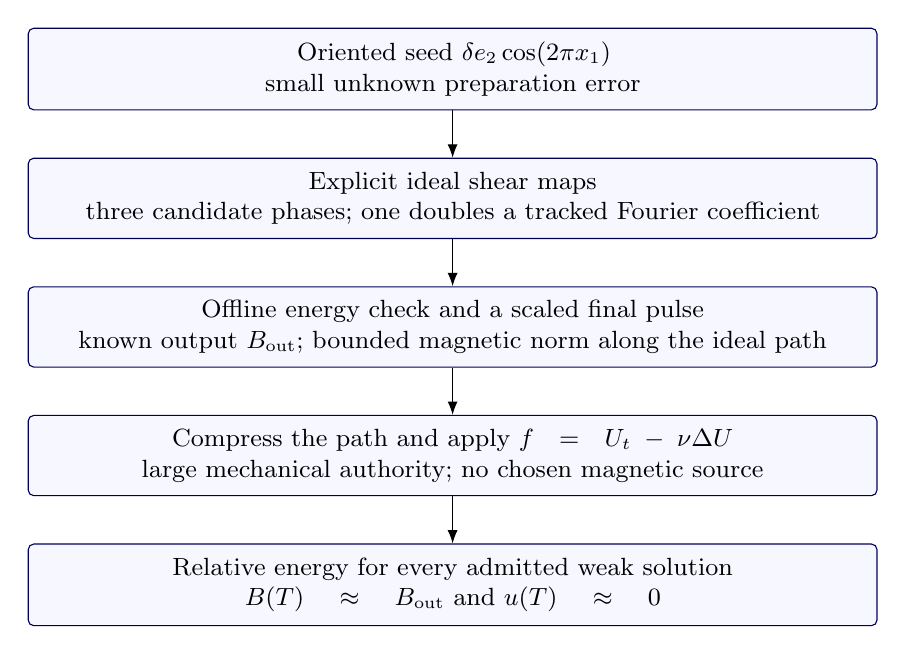
\begin{tikzpicture}[node distance=6mm,>=Latex,
 box/.style={draw=blue!35!black,rounded corners=2pt,fill=blue!3,
 text width=.86\linewidth,align=center,inner sep=5pt,font=\small}]
\node[box] (seed) {Oriented seed $\delta e_2\cos(2\pi x_1)$\\small unknown preparation error};
\node[box,below=of seed] (ideal) {Explicit ideal shear maps\\three candidate phases; one doubles a tracked Fourier coefficient};
\node[box,below=of ideal] (stop) {Offline energy check and a scaled final pulse\\known output $B_{\rm out}$; bounded magnetic norm along the ideal path};
\node[box,below=of stop] (force) {Compress the path and apply $f=U_t-\nu\Delta U$\\large mechanical authority; no chosen magnetic source};
\node[box,below=of force] (output) {Relative energy for every admitted weak solution\\$B(T)\approx B_{\rm out}$ and $u(T)\approx0$};
\draw[->] (seed)--(ideal);\draw[->] (ideal)--(stop);
\draw[->] (stop)--(force);\draw[->] (force)--(output);
\end{tikzpicture}
\end{center}

The important cancellation is in the \emph{pair} energy. Velocity and magnetic nonlinearities exchange energy; they need not be bounded separately in a strong norm. Against a smooth reference, the cubic perturbation terms cancel, leaving only known reference gradients and explicit residuals. Short physical time makes resistive diffusion, Lorentz mismatch and bounded additive errors small after their known amplification is paid.

There are two different ways to use this cancellation. With calibrated viscosity and a prepared pair, the complete smooth magnetic reference gives a strong output. Without viscosity compensation, pair energy remains bounded relative to the carrier, but the velocity error need not be small. A backward ideal test still predicts one terminal magnetic coefficient: derivatives fall on the known test rather than on the unknown magnetic field.

Other contracts are separated below: near-guide preparation uses supplied flux and a growing force bank; common erasure is Corollary~\ref{thm:ensemble}; joint targets with one signed magnetic channel remain conditional on Appendix~\ref{app:primitive}.
\clearpage



% ---- sections/03-setting ----
\section{Equations, solutions and resource conventions}\label{sec:setting}

Except in Section~\ref{sec:guide}, the domain is $\T^3=(\R/\Z)^3$ with normalized volume and $\kappa=2\pi$. Let $H^s_\sigma$ denote the real, mean-zero, divergence-free Sobolev fields, and put $\Hcal^s=H^s_\sigma\times H^s_\sigma$. Norms of pairs are Euclidean sums of squared component norms. The periodic Leray projection is $\PP$; at nonzero Fourier frequency $k$ its matrix is $I-k\otimes k/|k|^2$. We write
\[
 \Bcal(v,w)=\PP((v\cdot\nabla)w),\qquad
 \Ccal_v b=[v,b]=(v\cdot\nabla)b-(b\cdot\nabla)v.
\]
For $\nu,\rho>0$ the controlled equations are
\begin{align}
 u_t+\Bcal(u,u)-\Bcal(B,B)&=\nu\Delta u+f+h_u,\label{eq:mom}\\
 B_t+\Ccal_uB&=\rho\Delta B+j+h_B.\label{eq:ind}
\end{align}
The chosen force $f$ acts on momentum. A chosen induction source $j$ is present only when explicitly stated. The unknown disturbances $h=(h_u,h_B)$ are not controls. All are solenoidal and have zero mean. Thus both means are conserved; the guide-field section specifies a different magnetic mean.

\begin{definition}[Admitted realization]\label{def:LH}
An admitted realization is a distributional solution $(u,B)\in L^\infty(0,T;\Hcal^0)\cap L^2(0,T;\Hcal^1)$ with weakly continuous $L^2$ representatives and the Leray--Hopf total-energy inequality. We use these representatives at endpoints. If an endpoint is specified through a one-sided total-energy trace, that trace is required to be energy-admissible. The estimates below hold for it as well.
\end{definition}

There is at least one such solution for every datum and force used here; Appendix~\ref{app:weak} recalls the Galerkin argument. No weak uniqueness is assumed. For common erasure, strong continuation and the all-realization transfer come from the companion theorem. The conditional prefix construction also uses weak--strong uniqueness only with identical actual coefficients, forces and disturbances.

\begin{definition}[Finite description and polynomial resources]\label{def:resources}
Rational data and finite Fourier lists are encoded in binary. Their complete length is $L$, including all frequencies, numerators and denominators. A force description lists rational interval endpoints and ordinary rational polynomials in physical time multiplying the stated fixed spatial fields. A numerical resource bound $AR^p$ has fixed effectively computable $A,p$ and includes tolerance reciprocals, force peaks and impulses in $W^{1,\infty}$, and any additional physical quantities explicitly claimed. A digital bound $A(L+R)^p$ includes bit operations, working memory, output length, interval count and individual rational heights. Fixed precomputation is included.
\end{definition}

These are polynomial bounds in \emph{numerical inverse accuracies}, often called pseudopolynomial bounds. A bound polynomial in $\delta^{-1}$ is not a bound polynomial in the number of binary digits of $\delta$. Descriptions of output fields below consist of explicit shear maps or finite flow programs, rather than an uncharged solution operator for the physical equations.

The six mechanical modes of the main results are the sine/cosine partners of
\begin{equation}\label{eq:six}
 F_0=e_3\sin\kappa(x_1-x_2),\quad
 F_1=e_1\sin\kappa(x_2-x_3),\quad
 F_2=e_2\sin\kappa(x_3-x_1).
\end{equation}
They differ from the twelve fundamental modes
\begin{equation}\label{eq:twelve}
 \mathcal E=\operatorname{span}_{\R}
 \{e_i\sin\kappa x_j,e_i\cos\kappa x_j:i\ne j\}
\end{equation}
used in Section~\ref{sec:ensemble} and in the conditional one-channel extension. A translation or phase of one of these shears lies in its own sine/cosine pair and creates no new mechanical mode.



% ---- sections/04-main ----
\section{The six-mode preparation theorems}\label{sec:main}

Set $b_*=e_2\cos\kappa x_1$. An oriented seed is a genuine preparation resource: the invariant input $B=0$ cannot be turned into a nonzero field by momentum forcing alone.

\begin{theorem}[Prepared magnetic field and kinetic recovery]\label{thm:main}
There are fixed effectively computable constants $A,p$ and a total deterministic algorithm with the following property. Given rational $0<\nu\le1$, $0<\delta\le1$ and $0<\epsilon<1$, it returns rational $T,r>0$, a force $f$ on the six modes \eqref{eq:six} with rational piecewise-polynomial coefficients of degree at most six, and an explicit volume-preserving shear composition $\Phi$ of length $n=O(\log(2/\delta))$. Define
\[
 B_{\rm out}=\delta\push\Phi b_*.
\]
The compiler also supplies the evaluation representation in Lemma~\ref{lem:compiledquery}. The field $B_{\rm out}$ has norm in $(67/16,77/16]$. For every $0<\rho\le1$, every initial pair satisfying
\begin{equation}\label{eq:prepball}
 \norm{(u_0,B_0-\delta b_*)}_2\le r,
\end{equation}
every disturbance with $\norm h_{L^\infty\Hcal^0}\le1$, and every admitted realization of \eqref{eq:mom}--\eqref{eq:ind} with $j=0$, one has
\begin{align}
 \norm{(u(T),B(T)-B_{\rm out})}_2&\le\epsilon,\label{eq:mainout}\\
 4\le\norm{B(T)}_2\le5,\qquad
 \sup_{0\le t\le T}\norm{B(t)}_2&\le5.\label{eq:mainnorm}
\end{align}
For $R=2+\delta^{-1}+\epsilon^{-1}$, the quantities $T^{-1},r^{-1}$, the force peak and impulse in $W^{1,\infty}$, its essential time-derivative peak, the kinetic-energy reserve and the positive mechanical work have bounds $AR^p$. Digital resources have bounds $A(L+R)^p$. At rational coordinates, the field $B_{\rm out}$ and each fixed finite order of its spatial derivatives can be evaluated to a specified absolute accuracy using bit work polynomial in $n$, the coordinate description and the requested number of accuracy digits.
\end{theorem}

The algorithm knows $\nu$ and is independent of $\rho$. The output is a known field chosen by the algorithm; it is not an arbitrary requested magnetic pattern. The endpoint time is chosen by the algorithm. The following theorem earns different quantifiers by asking for less at that endpoint.

\begin{theorem}[A common magnetic output with unknown diffusivities]\label{thm:unknown}
Given rational $M\ge1$ and $0<\delta\le1$, a total deterministic algorithm returns rational $T,r>0$ and one force on \eqref{eq:six}, with rational piecewise-polynomial coefficients of degree at most five, such that
\begin{equation}\label{eq:unknownout}
 \norm{B(T)}_2\ge1
\end{equation}
for every $0<\nu,\rho\le1$, every $\norm{u_0}_2\le M$ and $\norm{B_0-\delta b_*}_2\le r$, every unit $L^\infty\Hcal^0$ disturbance, and every admitted realization. Numerical resources listed in Theorem~\ref{thm:main} have fixed polynomial bounds in $2+M+\delta^{-1}$, and digital resources in $L+2+M+\delta^{-1}$. This theorem does not assert kinetic recovery or full-field magnetic accuracy.
\end{theorem}

\begin{remark}[Calibration and absolute errors]\label{rem:calibration}
If Theorem~\ref{thm:main} is compiled with $\nu_c$ but the actual viscosity is $\nu_a$, the additional integrated residual is at most $Cn|\nu_a-\nu_c|$. Its final effect is at most $Cn e^{Cn}|\nu_a-\nu_c|$ after enlarging a fixed $C$. Thus a paid inverse-polynomial calibration interval suffices. No acquisition procedure for this interval or the seed is supplied. Unit \emph{absolute} disturbance is also not fixed fractional actuator error: the required force grows as the seed shrinks.
\end{remark}

Theorems~\ref{thm:main} and~\ref{thm:unknown} follow from three ingredients: energy comparison, an ideal finite shear program, and a finite-resource realization. We prove these in that order.

\begin{table}[htbp]
\caption{The operations have different contracts. A common force is one prescribed force for the whole stated uncertainty class.}\label{tab:contracts}
\small
\begin{tabular}{@{}p{.20\linewidth}p{.36\linewidth}p{.38\linewidth}@{}}
\toprule
Result & Input and force space & Endpoint and extra conditions\\
\midrule
Theorem~\ref{thm:main} &
Prepared oriented seed; six mechanical modes &
Known order-one magnetic field, small total velocity; calibrated $\nu$, common over $0<\rho\le1$\\[4pt]
Theorem~\ref{thm:unknown} &
Prepared seed, arbitrary bounded velocity; same six modes &
A magnetic Fourier output; common over $0<\nu,\rho\le1$, without kinetic recovery\\[4pt]
Theorem~\ref{thm:guide} &
Supplied nonzero guide; growing mechanical bank &
Chosen small analytic magnetic pattern; paid calibration and passive waiting\\[4pt]
Corollary~\ref{thm:ensemble} &
Unknown $H^1$ pair ball; twelve mechanical modes &
Chosen velocity and small magnetic field; common parameter rectangle; consequence of \cite[Theorem~2.2]{CommonControl}\\[4pt]
Theorem~\ref{thm:channel} &
Same ball and twelve modes, plus one signed magnetic channel &
Chosen joint Fourier target; known coefficients; conditional on the smooth-prefix hypothesis $\Qcal$\\
\bottomrule
\end{tabular}
\end{table}



% ---- sections/05-energy ----
\section{Relative energy and the rapid-induction principle}\label{sec:energy}

\subsection{Why the pair is the correct comparison object}
The Lorentz force cannot in general be estimated from magnetic energy in $H^{-1}$; Section~\ref{sec:obstructions} gives a counterexample. Fortunately, it is unnecessary to estimate that force separately. Its leading interaction with the velocity error cancels the corresponding induction interaction in the \emph{sum} of the two error energies.

\begin{lemma}[Comparison with a smooth approximate pair]\label{lem:relative}
Let $(U,b)$ be a smooth solenoidal pair, with the same means as an admitted realization, and define its residuals by
\begin{align*}
 R_u&=U_t+\Bcal(U,U)-\Bcal(b,b)-\nu\Delta U-f,\\
 R_B&=b_t+\Ccal_Ub-\rho\Delta b-j.
\end{align*}
Set $G=\norm{\nabla U}_\infty+\norm{\nabla b}_\infty$, with the Euclidean operator norm on gradients. Then, at every admitted trace,
\begin{equation}\label{eq:relative}
 \norm{(u-U,B-b)(t)}_2
 \le e^{\int_0^tG}
 \left[\norm{(u-U,B-b)(0)}_2+
 \int_0^t\big(\norm{(R_u,R_B)}_2+\norm h_2\big)\,ds\right].
\end{equation}
Known residuals need only be integrable in $L^2$; piecewise smooth references with matching values are allowed.
\end{lemma}

\begin{proof}
Write $v=u-U$ and $d=B-b$. For smooth solutions, subtract the equations and pair them with $v,d$. Advection by divergence-free fields integrates to zero. The three perturbation terms involving two unknown factors and one unknown derivative cancel by integration by parts. The remaining reference-gradient terms are
\[
 -\ip{v\cdot\nabla U}{v}+\ip{d\cdot\nabla U}{d}
 +\ip{d\cdot\nabla b}{v}-\ip{v\cdot\nabla b}{d}.
\]
Their absolute sum is at most $G(\norm v_2^2+\norm d_2^2)$. Dropping positive dissipation gives, for $z^2=\norm v_2^2+\norm d_2^2$,
\[
 \tfrac12(z^2)'\le Gz^2+
 \big(\norm{(R_u,R_B)}_2+\norm h_2\big)z.
\]
Use $(z^2+\alpha^2)^{1/2}$ and let $\alpha\downarrow0$. Integrating proves \eqref{eq:relative}. For an admitted weak solution, test the weak equations against $U,b$ and add the total-energy inequality. Every mixed term just displayed is well defined because the reference is smooth. Approximation in time gives the integrated inequality; weak lower semicontinuity extends it to the stated traces. This argument does not select a strong physical solution.
\end{proof}

\subsection{Weak observations require less preparation}
Let $w(s)$ be a prescribed smooth solenoidal carrier on $0\le s\le S$, with $w(0)=w(S)=0$. Its ideal induction propagator is $\Mcal_w(s,r)$, defined by $b_s+\Ccal_wb=0$. In particular, it is a known transport and stretching operation, not the propagator of the nonlinear physical system.

\begin{theorem}[Rapid realization of ideal magnetic observations]\label{thm:rapid}
Put $a=S/T$, $U(t)=aw(at)$ and choose
\begin{equation}\label{eq:rapidforce}
 f=a^2\big(w_s+\Bcal(w,w)\big)(at)-\nu a\Delta w(at),
 \qquad j_{\rm phys}(t)=a j_0(at).
\end{equation}
Suppose $\norm{(u_0,B_0)}_2\le M$. Define
\begin{align*}
 A_w&=\int_0^S\norm{\nabla w(s)}_\infty ds,&
 J&=\int_0^S\norm{j_0(s)}_2ds,\\
 H&=\int_0^T\norm{h(t)}_2dt,&
 Y&=e^{A_w}(M+J+H).
\end{align*}
Let $b_s+\Ccal_wb=j_0$, $b(0)=B_0$. For a smooth, possibly complex test $\psi$, let
\[
 \phi(s)=\Mcal_w(S,s)^*\psi,\qquad
 D_0=\sup_s\norm\phi_2,\quad
 D_1=2\sup_s\norm{\nabla\phi}_\infty,\quad
 D_2=\sup_s\norm{\Delta\phi}_2.
\]
Every admitted realization satisfies $\sup_t\norm{(u-U,B)}_2\le Y$ and
\begin{equation}\label{eq:rapiderror}
 \abs{\ip{B(T)-b(S)}\psi}
 \le TD_1Y^2+\rho TD_2Y+D_0\norm{h_B}_{L^1L^2}.
\end{equation}
If the viscous compensation is omitted in \eqref{eq:rapidforce}, the same conclusions hold after adding
\begin{equation}\label{eq:viscdefect}
 \overline\nu\int_0^S\norm{\Delta w(s)}_2ds
\end{equation}
inside the parentheses defining $Y$, uniformly for $0<\nu\le\overline\nu$.
\end{theorem}

\begin{proof}
Apply the pair-energy argument against $(U,0)$. Its only prescribed magnetic term is $a j_0(at)$. Integration gives the asserted bound $Y$. In the uncompensated case the smooth momentum residual is $-\nu\Delta U$, whose time integral is exactly bounded by \eqref{eq:viscdefect}. This term is independent of $T$, and is not claimed to vanish.

The adjoint satisfies
\[
 -\phi_s=w\cdot\nabla\phi+(\nabla w)^\mathsf T\phi.
\]
Test actual induction against $\phi(at)$ and subtract ideal induction. The prescribed source cancels. With $v=u-U$, periodicity gives
\begin{equation}\label{eq:weakbracket}
 \abs{\ip{\Ccal_vB}\phi}
 \le2\norm{\nabla\phi}_\infty\norm v_2\norm B_2.
\end{equation}
Diffusion is paired with $\Delta\phi$, so no physical derivative of $B$ is needed. Integrating these two terms and the magnetic disturbance proves \eqref{eq:rapiderror}. All tests are smooth; the same calculation is valid in the weak formulation. No solenoidal projection is required on $\phi$, since induction has no pressure. Standard differentiated characteristics give finite bounds for $D_i$ from supplied fixed-order derivatives of $w$.
\end{proof}

The theorem applies to an unknown input $B_0$ as a comparison principle, but does not reveal that input. Its constructive use below has a known central seed and an explicit preparation-error allowance. Estimate \eqref{eq:rapiderror} controls the selected smooth observations; it is not a strong-norm approximation.



% ---- sections/06-ideal ----
\section{A finite ideal program: growth, computation and stopping}\label{sec:ideal}

\subsection{An exact Fourier row}
Write $\widehat b(k)=\int_{\T^3}b(x)e^{-i\kappa k\cdot x}\,dx$. Let
\[
 \ell_0=e_1,\quad p_0=(e_1-e_2)/\sqrt2,
\]
and obtain $(\ell_j,p_j)$ by cyclic permutation of coordinates, with period three. The tracked observation at step $j$ is $Y_j=p_j\cdot\widehat b_j(\ell_j)$.

Use the nonnegative unit-integral pulse
\begin{equation}\label{eq:bump}
 q(s)=140s^3(1-s)^3\quad(0\le s\le1),
 \qquad q(s)=0\quad\hbox{otherwise}.
\end{equation}
It is globally $C^2$. A phase $\varphi$ in $F_0$ means $e_3\sin\kappa(x_1-x_2+\varphi)$, and similarly for the cyclic shears.

\begin{lemma}[Ideal row; zero-resistivity case of \cite{Rowan}]\label{lem:row}
For one unit-dose pulse of the $j$th cyclic shear,
\begin{equation}\label{eq:row}
 Y_{j+1}=-\pi Y_j e^{-i\kappa\varphi}+c_j+d_j e^{i\kappa\varphi},
\end{equation}
where $c_j,d_j$ depend on the incoming field but not on $\varphi$.
\end{lemma}

\begin{proof}
It suffices to treat $F_0$. Since this shear is independent of $x_3$, vertical Fourier modes do not interact. Only the vertical-zero projection $\beta$ enters $\widehat b(e_2)$. On this projection advection vanishes, $\beta_1,\beta_2$ are constant during the pulse, and
\[
 \beta_3(1)=\beta_3(0)+\kappa(\beta_1(0)-\beta_2(0))
 \cos\kappa(x_1-x_2+\varphi).
\]
The $e_2$ Fourier coefficient of the added term has contributions from incoming frequencies $e_1$ and $-e_1+2e_2$. Pairing with $(e_2-e_3)/\sqrt2$ gives the coefficient $-\kappa/2=-\pi$ on $Y_0e^{-i\kappa\varphi}$. The unchanged incoming $e_2$ coefficient and the other incoming frequency form $c_0$ and $d_0e^{i\kappa\varphi}$. Cyclic permutation proves the claim. No finite-dimensional Fourier closure is being assumed.
\end{proof}

\begin{lemma}[Three deterministic choices]\label{lem:phases}
For arbitrary complex $a,b,c$,
\begin{equation}\label{eq:threephase}
 \frac13\sum_{l=0}^2
 \abs{ae^{-2\pi il/3}+b+ce^{2\pi il/3}}^2
 =|a|^2+|b|^2+|c|^2.
\end{equation}
Consequently, if each of the three candidate observations in \eqref{eq:row} is calculated to error at most $\delta/128$, selecting the largest computed modulus gives
\begin{equation}\label{eq:double}
 |Y_{j+1}|\ge\pi|Y_j|-\delta/64\ge2|Y_j|
 \quad\hbox{whenever }|Y_j|\ge\delta/4.
\end{equation}
\end{lemma}

\begin{proof}
Expanding the squares in \eqref{eq:threephase}, every cross term contains a nonconstant character of the three roots of unity and sums to zero. Some candidate therefore has modulus at least $|a|$. Choosing an approximate maximum loses at most twice the calculation error. Apply this with $a=-\pi Y_j$, using $\pi>3$.
\end{proof}

\begin{example}[Why a single attractive phase can fail]\label{ex:cancellation}
If $Q(\varphi)=e^{-2\pi i\varphi}-1$, then $Q(0)=0$ although its extremal Fourier coefficient is one. At phases $1/3$ and $2/3$, $|Q|=\sqrt3$. The three-point average of $|Q|^2$ is two. Thus the phase choice protects against \emph{exact cancellation}; a lower bound on the size of one incoming term would not protect a fixed phase.
\end{example}

For $b_0=\delta b_*$, $|Y_0|=\delta/(2\sqrt2)\ge\delta/4$. Hence at most $\lceil\log_2(16/\delta)\rceil$ chosen unit pulses give $|Y_n|\ge4$.

\subsection{The calculation does not hide a many-body solver}
One ideal pulse has the explicit map
\begin{equation}\label{eq:shearmap}
 S(x)=x+d\sin\kappa(k\cdot x+\varphi),\qquad d\cdot k=0.
\end{equation}
It has determinant one and inverse obtained by reversing $d$. If $\Phi$ is a composition of $j$ such maps, ideal induction gives $b=\delta\push\Phi b_*$. Thus a candidate observation is exactly
\begin{equation}\label{eq:coefficientintegral}
 \int_{[0,1]^3}p\cdot D\Phi(x)\,\delta b_*(x)
 e^{-i\kappa\ell\cdot\Phi(x)}\,dx.
\end{equation}
The integrand is evaluated by elementary shear maps and matrix products. No physical MHD evolution is solved.

\begin{lemma}[Finite cubature]\label{lem:cubature}
All phase choices in a word of length $n$ can be made with bit operations and memory bounded by a fixed polynomial in $L+\delta^{-1}$ when $n=O(\log(2/\delta))$.
\end{lemma}

\begin{proof}
Uniformly in the phases, $\norm{DS}\le16$ and $\norm{D^2S}\le128$. The chain rule gives
\begin{equation}\label{eq:mapbounds}
 \norm{D\Phi_j}_\infty\le16^j,\qquad
 \norm{D^2\Phi_j}_\infty\le16^{2j}.
\end{equation}
Indeed, the second-derivative recurrence is bounded by
$16\norm{D^2\Phi_j}+128\norm{D\Phi_j}^2$, and $16+128\le16^2$.
The gradient of the integrand in \eqref{eq:coefficientintegral} is at most $16\delta16^{2j}$. A uniform midpoint grid with
\[
 m=2^{14}16^{2n}
\]
cells per direction has error less than $\delta/512$ for every candidate. Here $n$ bounds the \emph{candidate word length}, including its new pulse. Evaluating each integrand to complex error at most $\delta/512$ gives total error less than $\delta/128$, since the cubature weights are positive and sum to one.

There are $m^3=2^{42}16^{6n}$ nodes. For $n=\lceil\log_2(32/\delta)\rceil$, this is at most $C\delta^{-24}$. Elementary interval series for sine and cosine, and interval approximations to $\sqrt2$, require $O(n+\log\delta^{-1})$ precision bits up to fixed constants. Use lifts of coordinates to $\R^3$; their magnitude is $O(n+1)$, so no uncertain modular reduction is needed. Sum common-dyadic approximants exactly. This avoids one new denominator per node. Three candidates at each of $n$ stages still have polynomial cost. Fixed higher derivatives obey analogous exponential-in-$n$ bounds by repeated chain rules.
\end{proof}

\subsection{Stop at a bounded field without stopping the carrier mid-pulse}
Amplification alone might produce a large overshoot. The following modification bounds the whole magnetic path while retaining a zero carrier at the terminal time.

\begin{lemma}[Offline energy clamp]\label{lem:clamp}
Using at most $n=\lceil\log_2(32/\delta)\rceil$ pulses, the ideal program can be chosen with each dose in $[0,1]$, with
\begin{equation}\label{eq:clampbounds}
 \norm{b(n)}_2\in(67/16,77/16],\qquad
 \sup_{s\le n}\norm{b(s)}_2\le77/16.
\end{equation}
Its phases and final rational dose are computable with fixed polynomial resources in $L+\delta^{-1}$.
\end{lemma}

\begin{proof}
Follow the deterministic unit-pulse word and calculate the norm after each candidate to absolute error at most $1/16$. Stop at the first computed norm greater than $17/4$. A stop must occur by step $n$: otherwise the unmodified row bound would give a terminal coefficient at least eight while every computed norm were at most $17/4$.

The preceding true norm is at most $69/16$. If the stopping computed norm is at most $19/4$, the new true norm lies in $(67/16,77/16]$ and the pulse is accepted. Otherwise its true norm exceeds $75/16$. Scale the \emph{entire} final bump by a dose $s\in[0,1]$. Do not cut the bump at the instant a threshold is reached: that would leave nonzero carrier velocity.

For the last shear $F$, volume preservation gives the exact quadratic energy
\begin{equation}\label{eq:energyquadratic}
 E(s)=\int|(I+sDF)b_{\rm prev}|^2
 =E_0+2sL+s^2Q,\qquad Q\ge0.
\end{equation}
The value $(9/2)^2$ lies strictly between $E(0)$ and $E(1)$. A finite rational dose suffices without dividing by $Q$. For example, let $K\ge\norm{DF}_\infty$ be a fixed integer, put
\[
 D=2(K+K^2)(69/16)^2,\qquad J\ge16\max(1,D),
\]
and compute $E(j/J)$ to error at most $1/16$. Choose the grid point whose computed energy is closest to $(9/2)^2$. The derivative bound $|E'|\le D$ and the two evaluation errors give true energy error at most $3/16$. Its norm lies in $[17/4,19/4]$, inside the required range.

The energy integrand has gradient bounded by $C\delta^2 16^{3n}$. Midpoint cubature and fixed-precision interval evaluation therefore still have polynomial cost in $\delta^{-1}$, although the exponent may exceed the coefficient-only cost in Lemma~\ref{lem:cubature}. Along each pulse the cumulative dose is monotone, since $q\ge0$. Convexity of \eqref{eq:energyquadratic} bounds its energy by the two endpoint energies. All earlier endpoints have norm at most $69/16$, and the accepted final endpoint at most $77/16$. Fill any unused normalized intervals with zero carrier. This proves \eqref{eq:clampbounds}.
\end{proof}

This clamp is used only in Theorem~\ref{thm:main}. Stopping on total energy would destroy the specific tracked-coefficient guarantee used to transfer Theorem~\ref{thm:unknown} through a weak test.



% ---- sections/07-realization ----
\section{Physical realization and the costs of compression}\label{sec:realization}

We first bound the known ideal word, then choose its physical clock, and only then round the emitted force. This order separates uniform analytic estimates from finite arithmetic. None of the bounds below requires solving the physical MHD equations.

\subsection{Effective bounds for the known word}
For a unit or smaller dose, write $S_s(x)=x+sF(x)$ for one of the shears in \eqref{eq:six}. Its induction action is
\begin{equation}\label{eq:onepulsepush}
 (M_sv)(x)=(I+sDF(y))v(y),\qquad y=S_s^{-1}(x).
\end{equation}
The inverse map is explicit because $F$ is constant on its own straight streamlines.

\begin{lemma}[Known-field and adjoint envelopes]\label{lem:wordenvelope}
There are effectively computable integers $K,d\ge1$, independent of the phases, doses, $n,\delta$ and physical diffusivities, with the following properties. For every word of at most $n$ pulses, its carrier $w$ and ideal field $\beta$ satisfy
\begin{align}
 \int_0^n(\norm{\nabla w}_\infty+\norm{\Delta w}_2)ds&\le Kn,
 &e^{Kn}&\le2^{dn},\label{eq:wordstrain}\\
 \sup_s\norm{\nabla\beta(s)}_\infty&\le K2^{dn},
 &\sup_s\norm{(\Bcal(\beta,\beta),\rho\Delta\beta)}_2
       &\le K2^{dn}\quad(0<\rho\le1).\label{eq:wordresidual}
\end{align}
For the unit-polarized terminal Fourier test used in Theorem~\ref{thm:unknown}, its ideal backward adjoint obeys
\begin{equation}\label{eq:adjointenvelope}
 \sup_s\big(\norm\phi_2+2\norm{\nabla\phi}_\infty
                         +\norm{\Delta\phi}_2\big)\le K2^{dn}.
\end{equation}
At each fixed higher order $m$ one also has
\begin{equation}\label{eq:referencebounds}
 \sup_s\big(\norm{\beta(s)}_{H^m}
       +\norm{\beta(s)}_{W^{m-2,\infty}}\big)
 \le C_m\delta L_m^n
\end{equation}
with fixed effective $C_m,L_m$.
\end{lemma}

\begin{proof}
Here is one entirely numerical majorant. Use the maximum of Euclidean Fr\'echet derivative norms for $C^m$. Since $|k|<2$ and $\kappa<7$, one has $\norm{D^rF}_\infty\le14^r$ and $\norm{D^rS_s^{\pm1}}_\infty\le15^r$ for $r\ge1$. Moreover $DF(S_s^{-1}x)=DF(x)$. The chain-rule partition count is at most $(m+1)^{m+1}$ and the Leibniz binomial sum at most $2^m$. Thus, for example,
\begin{equation}\label{eq:explicitLm}
 L_m=2^{m+2}15^{2m+2}(m+1)^{m+1}
\end{equation}
bounds both the pushforward and the adjoint pulse on $C^m$, for every phase and $|s|\le1$. Applying this estimate successively proves \eqref{eq:referencebounds}; the finitely many tensor-to-Sobolev norm factors are bounded by direct sums over multi-indices.

Specifically $\norm{b_*}_{C^2}\le49$, so $\norm\beta_{C^2}\le49\delta L_2^n$. Hence $\norm{\nabla\beta}_\infty\le49L_2^n$, $\norm{\Delta\beta}_2\le147L_2^n$, and $\norm{\Bcal(\beta,\beta)}_2\le2401L_2^{2n}$, using $\delta\le1$ and the $L^2$ contraction of $\PP$. The sum of single-pulse strain and Laplacian integrals is at most $14+98=112$, since the nonnegative bump has mass one.

There is also an explicit adjoint. If $\Phi_{n,s}$ is the volume-preserving map from normalized time $s$ to $n$, then
\[
 \phi(s,y)=D\Phi_{n,s}(y)^{\mathsf T}
                    \psi(\Phi_{n,s}(y)).
\]
This follows by a change of variables in the pushforward pairing. Equivalently apply the adjoints of the individual pulses in reverse order. Their $C^2$ bound is also $L_2$, and $\norm\psi_{C^2}\le49$, so the left side of \eqref{eq:adjointenvelope} is at most $294L_2^n$. Consequently the fixed integer choices
\begin{equation}\label{eq:explicitKd}
 K=4096,\qquad d=2K+2\lceil\log_2L_2\rceil+4
\end{equation}
suffice for all displayed estimates, including $e^{Kn}\le2^{dn}$. These deliberately loose values make the proof reproducible; they are not efficiency estimates.
\end{proof}

\subsection{A complete clock choice for full-field preparation}
Let $w$ be the clamped word, $\beta(0)=\delta b_*$ and $\beta_s+\Ccal_w\beta=0$. Set
\begin{equation}\label{eq:maincarrier}
 a=n/T,\qquad U(t)=aw(at),\qquad b(t)=\beta(at),
\end{equation}
and first consider the exact force
\begin{equation}\label{eq:mainforce}
 f_*=U_t-\nu\Delta U.
\end{equation}
Only one shear is active, so $\Bcal(U,U)=0$. Thus the reference residuals are exactly
$R_u=-\Bcal(b,b)$ and $R_B=-\rho\Delta b$. The physical force does not cancel the Lorentz feedback.

\begin{lemma}[Uniform error with a paid force approximation]\label{lem:rapidbudget}
Let $\norm{f-f_*}_{L^\infty L^2}\le\theta$, $\norm h_{L^\infty\Hcal^0}\le1$, and let the initial pair error be at most $r$. With $K,d$ as in Lemma~\ref{lem:wordenvelope}, every admitted realization satisfies
\begin{equation}\label{eq:fullbound}
 \sup_{t\le T}\norm{(u-U,B-b)(t)}_2
 \le e^{Kn+TK2^{dn}}
          \big[r+T K2^{dn}+T(1+\theta)\big].
\end{equation}
In particular, for $\epsilon_*=\min(\epsilon,1/8)$, the rational choices
\begin{equation}\label{eq:clockA}
 D_A=2d+4,\qquad
 T=r=\frac{\epsilon_*}{256K}\,2^{-D_A n},
 \qquad\theta\le1/16
\end{equation}
make this error smaller than $\epsilon_*/16$, uniformly for every $0<\rho\le1$.
\end{lemma}

\begin{proof}
Lemma~\ref{lem:relative} and \eqref{eq:wordstrain}--\eqref{eq:wordresidual} give \eqref{eq:fullbound}. The force approximation is another momentum residual and is not multiplied by its inverse time scale a second time. Under \eqref{eq:clockA}, $TK2^{dn}\le1/256$, so its exponential is at most two. Also $1+\theta\le2K2^{dn}$. The right-hand side is therefore at most
\[
 2^{dn+1}\big[r+3TK2^{dn}\big]
 \le\frac{\epsilon_*}{128}
       \left[2^{-(D_A-d)n}+3\,2^{-(D_A-2d)n}\right]
 <\epsilon_*/16.
\]
We used $K\ge1$ and $n\ge1$. This proves a concrete sufficient choice rather than an unspecified asymptotic clock.
\end{proof}

At $U(T)=0$, the last lemma proves \eqref{eq:mainout}. The clamp bounds imply final norm at least $67/16-1/8>4$ and norm throughout at most $77/16+1/8<5$. The smaller error just proved leaves slack for the stated margins.

\subsection{A common output without viscosity compensation}
For the unclamped word set $f_*=U_t$. Its uncompensated viscous defect has time integral
\[
 \nu\int_0^T\norm{\Delta U}_2dt
 =\nu\int_0^n\norm{\Delta w}_2ds\le Kn;
\]
The Laplacian bound is included in Lemma~\ref{lem:wordenvelope}. Let $H=M+Kn+4$. Relative energy against $(U,0)$ gives
\begin{equation}\label{eq:Yunknown}
 \sup_{t\le T}\norm{(u-U,B)(t)}_2\le2^{dn}H
\end{equation}
for every $0<\nu,\rho\le1$, if $r,T\le1$ and $\theta\le1/16$. In Theorem~\ref{thm:rapid}, the initial discrepancy from the central seed contributes at most $K2^{dn}r$. Equations \eqref{eq:adjointenvelope} and \eqref{eq:Yunknown} therefore give
\begin{equation}\label{eq:weakunknownerror}
 |Y_n^{\rm actual}-Y_n^{\rm ideal}|
 \le K2^{3dn}\big[r+4TH^2\big].
\end{equation}
This follows term by term from $Y^2$, $\rho Y$, the unit magnetic disturbance, and the reserved force approximation; $H\ge1$ absorbs the lower powers. Choose
\begin{equation}\label{eq:clockB}
 D_B=3d+4,\qquad
 r=\frac{2^{-D_Bn}}{256K},\qquad
 T=\frac{2^{-D_Bn}}{256KH^2}.
\end{equation}
Then \eqref{eq:weakunknownerror} is at most $5\,2^{-4n}/256<1/2$. Since $|Y_n^{\rm ideal}|\ge4$, the actual norm exceeds one. This proves the endpoint of Theorem~\ref{thm:unknown} with one force for the entire parameter and data class. No parameter-dependent exceptional event is used. The velocity reserve in \eqref{eq:Yunknown} is not a kinetic-recovery conclusion.

\subsection{A finite-bit compiler for the force itself}
On a physical interval $I_j=[j/a,(j+1)/a]$, the force \eqref{eq:mainforce} is a combination of the two fixed quadratures of one shear, with scalar factors
\[
 a^2 s_j q'(at-j),\qquad
 \nu\kappa^2|k_j|^2a s_j q(at-j),
 \quad 0\le s_j\le1.
\]
Here $s_j$ and every knot are rational, while the phase factors are elementary computable constants.

\begin{lemma}[Rational pulse compilation]\label{lem:pulsebits}
For $a\ge1$ and rational $0<\theta\le1$, rational coefficients can be produced with
$\norm{f-f_*}_{L^\infty W^{1,\infty}}\le\theta$.
If $\ell(a)$ is the binary length of the rational clock factor $a$, each coefficient and knot has binary length at most
\begin{equation}\label{eq:pulsebitheight}
 C\big[L+\ell(a)+\log_2(n+2)+\log_2(\theta^{-1}+2)\big].
\end{equation}
There are at most $Cn$ coefficients of degree at most six. In the uncompensated construction the degree is at most five.
\end{lemma}

\begin{proof}
Expand the phase into sine and cosine partners. Round once the scalar multipliers of $a^2q'$ and $aq$ to a common $b$-bit dyadic grid. Fixed spatial norms and pulse norms give
$\norm{f-f_*}_{W^{1,\infty}}\le C a^2 2^{-b}$.
Thus $b=\lceil\log_2(Ca^2/\theta)\rceil+2$ suffices. Elementary interval evaluation of $\pi$, the three phase values and the known $\nu$ uses this precision plus guard bits; reading the exact rational $\nu$ costs its input length.

For a fixed polynomial degree $l\le6$, the exact expansion
\[
 (at-j)^l=\sum_{k=0}^l\binom lk a^k(-j)^{l-k}t^k
\]
increases rational numerator and denominator lengths by at most a fixed multiple of the bit length of $a$ and $\log_2(n+2)$. It is a constant number of rational operations per coefficient. The knots $j/a$ have the same height bound. Round in the local pulse basis before this expansion; then the zeros of $q,q',q''$ at the joins are preserved exactly. The degree assertions follow from the degrees of $q$ and $q'$.
\end{proof}

For the clocks \eqref{eq:clockA} and \eqref{eq:clockB}, exact rational arithmetic gives $\ell(a)\le C[L+n+\log_2(M+2)]$, with $M$ omitted in the prepared case. Thus numerical magnitude is not being substituted for rational bit height. Take $\theta=1/16$ in the preceding lemma. The strong and weak error budgets already include it. This proves that the exact-reference argument really emits ordinary rational force coefficients.

\subsection{Physical and digital resources}
The unit-pulse norms, including their derivatives, give
\begin{align}
 \esssup_t\norm f_{W^{1,\infty}}&\le C(n/T)^2,
 &\int_0^T\norm f_{W^{1,\infty}}dt&\le Cn^2/T,\label{eq:forcesize}\\
 \esssup_t\norm{f_t}_{W^{1,\infty}}&\le C(n/T)^3.
\end{align}
The rational approximation has the same envelopes. Equations \eqref{eq:fullbound} or \eqref{eq:Yunknown} bound the actual velocity by $Cn/T$: in the second case, \eqref{eq:clockB} makes $2^{dn}H\le Cn/T$. Hence the kinetic-energy reserve is at most $C(n/T)^2$, and
\begin{equation}\label{eq:work}
 \int_0^T\max\{\ip{f(t)}{u(t)},0\}\,dt\le Cn^3/T^2.
\end{equation}
For $n=\lceil\log_2(32/\delta)\rceil$, one has $2^n\le64/\delta$. Substitution into \eqref{eq:clockA} and \eqref{eq:clockB} turns every time or tolerance reciprocal into a fixed power of $\delta^{-1}$, multiplied only by powers of $\epsilon^{-1}$ or $M+n$. The force and work bounds are then polynomial in the numerical resources stated in the main theorems. Lemmas~\ref{lem:cubature}, \ref{lem:clamp} and \ref{lem:pulsebits} give their separate complete bit bounds.

\begin{lemma}[Evaluation of the compiled output]\label{lem:compiledquery}
The output representation can be chosen so that, after compilation, $B_{\rm out}$ and any fixed derivative can be evaluated at a rational point of description length $L_x$ to error $2^{-b}$ in bit work polynomial in $n,L_x,b$. The compiler also pays for the seed coefficient's full original bit length.
\end{lemma}

\begin{proof}
First apply the inverse shears to obtain $y=\Phi^{-1}(x)$ and then compute $D\Phi(y)\delta b_*(y)$ by forward products. Fixed-order errors amplify by at most $L_m^n$, so $b'=b+C_mn+C_m$ accuracy digits suffice for all elementary evaluations. Each shear has a phase from a fixed set and a dose from the fixed clamp grid, so the word description has length $O(n)$.

One must also specify access to $\delta$: a short numerical value can have a long rational denominator. Let $L_\delta$ be its original rational description length. During compilation, compute its first $L_\delta$ binary fractional digits by exact long division, and store them after the shear list, followed by a delimiter and the original exact rational. This takes polynomial work in $L_\delta$ and adds $O(L_\delta)$ output bits, already covered by the compilation bound. Include its integer bit; $\delta\le1$.

The evaluator reads only the first $b'$ digits when the delimiter has not yet appeared; their truncation error is at most $2^{-b'}$. If it reaches the delimiter first, then $L_\delta\le b'$ and reading and dividing the exact fallback rational also has cost polynomial in $b'$. Thus a query does not silently reread an arbitrarily long seed denominator. This streamable trusted output format proves the asserted bound and works for every fixed derivative order with its corresponding guard digits.
\end{proof}



% ---- sections/08-guide ----
\section{A different operation: preparation near a supplied guide}\label{sec:guide}

The six-mode theorem chooses its own magnetic output. To choose a magnetic pattern, one can instead supply nonzero mean flux and allow the mechanical actuator bank to grow with spatial accuracy. This section uses that different contract. Work on $(\R/2\pi\Z)^3$, still with normalized volume, so Fourier differentiation has multiplier $ik$.

\subsection{An induction inverse on a volume-preserving orbit}
Suppose a constant vector $\beta$ satisfies, for fixed $q$ and $\gamma>0$,
\begin{equation}\label{eq:dioph}
 |\beta\cdot k|\ge\gamma |k|_1^{-q}\qquad(k\in\Z^3\setminus\{0\}).
\end{equation}
Let $D_\beta=\beta\cdot\nabla$.

\begin{proposition}[Orbit inverse]\label{prop:inverse}
If $\Phi$ is a smooth volume-preserving diffeomorphism isotopic to the identity and $B=\push\Phi\beta$, then
\begin{equation}\label{eq:RB}
 R_Bg=\push\Phi D_\beta^{-1}\push{\Phi^{-1}}g
\end{equation}
is a right inverse of $v\mapsto[B,v]$ on smooth mean-zero solenoidal fields. It preserves reality, zero mean and solenoidality. For every fixed integer $r\ge0$,
\begin{equation}\label{eq:tameinverse}
 \norm{R_Bg}_{H^r}
 \le C_r\gamma^{-1}P_r(\mathcal G)\norm g_{H^{r+\lceil q\rceil}},
\end{equation}
where $\mathcal G$ bounds sufficiently many fixed derivatives of $\Phi,\Phi^{-1}$ and $P_r$ is a fixed polynomial.
\end{proposition}

\begin{proof}
For a periodic lift $\Phi(x)=x+\psi(x)$ and a solenoidal $v$,
\begin{equation}\label{eq:meanpush}
 \int\push\Phi v\,dy=\int D\Phi(x)v(x)\,dx
 =\int v+\int(v\cdot\nabla)\psi=\int v.
\end{equation}
Thus both pushforwards in \eqref{eq:RB} preserve the zero-mean domain on which $D_\beta^{-1}$ is defined. Its nonzero Fourier coefficients are $\widehat g(k)/(i\beta\cdot k)$. They satisfy \eqref{eq:tameinverse} by \eqref{eq:dioph} and the product and chain rules. Naturality of Lie brackets gives
$[B,R_Bg]=\push\Phi[\beta,D_\beta^{-1}\push{\Phi^{-1}}g]=g$.
\end{proof}

For an isotopy $\Phi_s$ beginning at the identity, put
\[
 B_s=\push{\Phi_s}\beta,\qquad
 W_s=(\partial_s\Phi_s)\circ\Phi_s^{-1}.
\]
Over physical time $T$, define
\begin{equation}\label{eq:guidevelocity}
 b_r(t)=B_{t/T},\qquad
 u_r(t)=T^{-1}W_{t/T}-\rho R_{B_{t/T}}\Delta B_{t/T}.
\end{equation}
Then, exactly,
\begin{equation}\label{eq:guideinduction}
 \partial_tb_r=\rho\Delta b_r+[b_r,u_r].
\end{equation}
Indeed, $\partial_sB_s=[B_s,W_s]$ and the inverse term cancels resistive diffusion. The complete momentum force is
\begin{equation}\label{eq:guideforce}
 f_r=(u_r)_t-\nu\Delta u_r+
 \Bcal(u_r,u_r)-\Bcal(b_r,b_r).
\end{equation}
Here the Lorentz work is explicitly paid, unlike the small residual retained in the rapid seed construction.

\subsection{A local target class and a robust finite operation}
For $a>0$, write $|H|_a$ for the supremum norm of a periodic holomorphic field in $|\Ima x_j|<a$. The following local-rigidity statement is classical in mechanism; a direct proof with the needed mean constraint is given in Appendix~\ref{app:analytic}.

\begin{lemma}[Fixed-mean analytic straightening]\label{lem:straightening}
For fixed $q$, there is an effective $c_q>0$ such that, for $0<a\le1$, a real analytic mean-zero solenoidal $H$ with
\begin{equation}\label{eq:analyticsmall}
 |H|_a\le c_q\gamma a^{100+q}
\end{equation}
satisfies $\beta+H=\push\Phi\beta$ for a volume-preserving analytic $\Phi$ isotopic to the identity. There is an isotopy to $\Phi$ with bounded fixed-order geometry and
\begin{equation}\label{eq:deformation}
 \int_0^1\norm{\nabla W_s}_\infty ds
 \le C_q\gamma^{-1}a^{-(q+34)}|H|_a\le1/4.
\end{equation}
The constants may be decreased to impose the last inequality.
\end{lemma}

An effective example is $\beta=\Lambda(1,\alpha,\alpha^2)$, where $\Lambda>0$ is rational and $\alpha$ is the real root of $\alpha^3-\alpha-1=0$. The other two algebraic conjugates have modulus less than one. For $k\ne0$, the algebraic norm of $k_1+k_2\alpha+k_3\alpha^2$ is a nonzero integer. Bounding its other two factors by $|k|_1$ proves \eqref{eq:dioph} with $q=2$ and $\gamma=\Lambda$.

\begin{definition}[Efficiently specified guide]\label{def:efficientguide}
For a computational resource assertion, the fixed guide is supplied with an algorithm returning rational approximations to its components within $2^{-b}$ in at most $C(b+1)^c$ bit operations. The geometric results above require only \eqref{eq:dioph}; the polynomial bit bounds below also require this evaluation condition. The cubic algebraic guide satisfies it: bisection of $x^3-x-1$ on $[1,3/2]$, where its derivative is at least two, uses $O(b)$ steps of polynomial-bit rational arithmetic.
\end{definition}

\begin{lemma}[Uniform reference norms before finite rounding]\label{lem:guidenorms}
Fix $a,q,\beta,\gamma$ as in Lemma~\ref{lem:straightening}. For every fixed spatial order $m$, all finite exact isotopies of its iteration have computable bounds
\begin{equation}\label{eq:guideuniform}
 \sup_s\left[
 \norm{B_s}_{C^m}
 +\sum_{i=0}^2\left(\norm{\partial_s^iW_s}_{C^m}
                  +\rho^{-1}\norm{\partial_s^iV_s}_{C^m}\right)
 \right]\le C_m,\qquad V_s=-\rho R_{B_s}\Delta B_s,
\end{equation}
independent of the number of stages and the target's raw Fourier support. Constants may depend on the fixed guide and strip. Choose a rational
$J_{\rm ref}\ge\sup_s(\norm{\nabla V_s}_\infty+\norm{\nabla B_s}_\infty)$
with $J_{\rm ref}\le C(1+\rho)$, and put $T=(1+J_{\rm ref})^{-1}$. The force \eqref{eq:guideforce} then satisfies
\begin{align}
 \norm{f_r}_{L^\infty H^m}
       &\le C_m(1+\nu)(1+\rho)^2,\label{eq:guideforcebound}\\
 \norm{\partial_tf_r}_{L^\infty H^m}
       &\le C_m(1+\nu)(1+\rho)^3.\label{eq:guideslewbound}
\end{align}
Time derivatives at joins are understood essentially.
\end{lemma}

\begin{proof}
The analytic estimates in Appendix~\ref{app:analytic} bound every fixed derivative of the $j$th generating field by
$C_m2^{c_mj}4^{-2^j}$. Time reparametrization on an interval of length $2^{-j-1}$ adds only another fixed power of $2^j$. These sequences have a computable summable majorant: once $2^j$ exceeds a fixed threshold, the ratio of successive terms is at most $1/2$; the preceding finite sum is bounded directly. Product and inverse-map rules therefore bound the geometry uniformly through every required fixed order.

The orbit inverse \eqref{eq:RB} has a fixed derivative loss. Apply its estimate at the finitely many orders needed for $\Delta B_s$ and two time derivatives. Differentiation of the pushforwards gives
\begin{equation}\label{eq:inverseprime}
 \partial_sR_{B_s}=-\Ccal_{W_s}R_{B_s}+R_{B_s}\Ccal_{W_s}.
\end{equation}
A second differentiation produces only finitely many such commutators, so it creates no new inverse or search. This proves \eqref{eq:guideuniform}. In physical time,
$u_r=T^{-1}W+V$ has spatial norms bounded by $C(T^{-1}+\rho)$, its first time derivative by $C(T^{-2}+\rho T^{-1})$, and its second by $C(T^{-3}+\rho T^{-2})$. Substitute these bounds into \eqref{eq:guideforce} and its derivative, and use $T^{-1}\le C(1+\rho)$. This proves \eqref{eq:guideforcebound}--\eqref{eq:guideslewbound}.
\end{proof}

\begin{lemma}[Guide calibration and error propagation]\label{lem:guidebudget}
Let a finite represented isotopy satisfy the bounds of Lemma~\ref{lem:guidenorms} and the strain bound $1/4$. Suppose its endpoint map and inverse are within $\chi$ in a sufficiently high fixed derivative norm of the exact target conjugacy. Let
\[
 \zeta=|\nu_a-\nu|+|\rho_a-\rho|+|\beta_a-\beta|\le1
\]
and let $\theta=\norm{f-f_r}_{L^\infty L^2}$. There is a known polynomial $P_{\rm cal}\le C(1+\nu+\rho)^3$, enlarged to include the fixed geometry constants, such that after an unforced initialization time $T_0$ and writing time $T$,
\begin{align}
 \norm{(u_{\rm final}-u_*,B_{\rm final}-B_*)}_2
 \le{}&8\left[Me^{-\mu_0T_0}+\frac{\eta}{\mu_0}
                 +T(\eta+\theta+P_{\rm cal}\zeta)\right]\notag\\
 &+C(1+\rho)\chi+C\zeta,\label{eq:guideerrorledger}
\end{align}
provided the actual diffusivities are at least $\mu_0$ and
$\zeta\le c_{\rm geo}$ for a fixed explicitly bounded positive $c_{\rm geo}$.
The conclusion holds for every admitted realization.
\end{lemma}

\begin{proof}
About the actual conserved mean $\beta_a$, the constant-guide Alfv\'en terms cancel from pair energy. Thus the fluctuation at the end of the wait is bounded by $Me^{-\mu_0T_0}+\eta/\mu_0$.

During writing compare to $(u_r,\push{\Phi_s}\beta_a)$, not to a magnetic reference with the wrong mean. Put $\delta B_s=\push{\Phi_s}(\beta_a-\beta)$. The induction residual, up to its immaterial sign, is the sum
\[
 (\rho_a-\rho)\Delta(\push{\Phi_s}\beta_a)
 +\rho\{\Delta\delta B_s-[\delta B_s,R_{B_s}\Delta B_s]\}.
\]
The momentum residual consists of $(\nu-\nu_a)\Delta u_r$, the difference of the two Lorentz quadratics, and the force error. Each is bounded in $L^2$ by $P_{\rm cal}\zeta+\theta$ using \eqref{eq:guideuniform} and $\zeta\le1$. The integrated reference gradient is at most $5/4+CT\zeta$; choose $c_{\rm geo}$ so that its exponential is below eight. Lemma~\ref{lem:relative} gives the bracketed term in \eqref{eq:guideerrorledger}. Product rules in \eqref{eq:RB} bound the endpoint map/inverse perturbation by $C(1+\rho)\chi$ and the endpoint mean discrepancy by $C\zeta$. This proves the displayed bound. In particular the actual guide need not itself satisfy a Diophantine condition.
\end{proof}

\begin{theorem}[Near-guide magnetic preparation]\label{thm:guide}
Fix an efficiently specified guide $\beta$, its exponent $q$, a rational lower constant $\gamma>0$, and a rational strip width $0<a\le1$ as above. Let $H$ be a rational finite Fourier target satisfying \eqref{eq:analyticsmall}. Given rational nominal coefficients $\nu,\rho>0$, $M\ge1$, a lower actual diffusivity bound $0<\mu_0\le\min(\nu,\rho)$ and $0<\epsilon<1$, there is a deterministic finite program using a target-dependent finite Fourier bank of mechanical forces and no chosen magnetic source, with the following properties.

It prepares $B_*=\beta+H$ and the compatible terminal velocity $u_*=-\rho R_{B_*}\Delta B_*$ to joint $L^2$ error $\epsilon$, from every unknown initial fluctuation of joint $L^2$ norm at most $M$ about the supplied guide. The assertion holds for every admitted realization, for sufficiently small explicitly paid absolute disturbances and sufficiently narrow calibrated intervals for $\nu,\rho$ and the actual guide mean. The total time includes passive initialization of length at most
$C\mu_0^{-1}\log(2+M/\epsilon)$ and a compiler-chosen writing time. With $q,a,\beta,\gamma$ fixed, the inverse tolerances, force and energy bounds, installed mode count, digital work and memory have fixed polynomial bounds in $L+2+M+\mu_0^{-1}+\nu+\rho+\epsilon^{-1}$.
\end{theorem}

The fixed-strip convention in this complexity statement is deliberate. The analytic estimates below display their strip dependence, but we do not assert a uniform bit-complexity theorem for vanishing input strip width. The full actuator bank and the nonzero guide energy are resources. In particular, this is not a twelve-actuator theorem or a zero-flux theorem.

\begin{proof}
We make each operation and error budget explicit. Set $\sigma=\epsilon/1024$ and choose $P\ge1$ to dominate the geometry and calibration constants in Lemma~\ref{lem:guidebudget}. Sufficient rational tolerances are
\begin{equation}\label{eq:guidechoices}
 \begin{aligned}
 T_0&=\mu_0^{-1}\left\lceil\log_2(M/\sigma)\right\rceil,&
 \eta&\le\sigma\min\{\mu_0,(1+T)^{-1}\},\\
 \theta&\le\sigma/(1+T),&
 \zeta&\le\min\{c_{\rm geo},\sigma/[P(1+T)]\},\\
 \chi&\le\sigma/[P(1+\rho)].
 \end{aligned}
\end{equation}
Use the displayed upper bounds or fixed rational fractions for the compiler's design tolerances; unnecessarily smaller tolerances would have their own costs. All input parameters here are rational; the logarithmic ceiling is found by binary comparisons, not by an exact-real operation. The first choice gives $Me^{-\mu_0T_0}\le\sigma$. The five contributions inside the square brackets of \eqref{eq:guideerrorledger} are then at most $\sigma$ each, and each endpoint correction is at most $\sigma$. Consequently the final error is at most $42\sigma<\epsilon$.

It remains to construct the represented isotopy and rational force within these budgets. Decrease the fixed smallness constant in \eqref{eq:analyticsmall} once so that the exact strain has a strict margin below $1/4$. Lemma~\ref{lem:finiteguide} in Appendix~\ref{app:finiteguide} constructs a finite composition of exact flows of stored rational solenoidal Fourier fields. Its endpoint and fixed derivatives approximate the exact analytic construction within $\chi$, including the required normalized-time derivatives. It therefore retains the strain and geometry margins. This step is a finite Fourier/flow calculation on known functions. It is not evolution of an unknown physical state.

Here is a concrete force discretization. Let $P_8\ge1$ and $P_t\ge1$ be rational bounds for $\norm{f_r}_{L^\infty H^8}$ and $\norm{\partial_tf_r}_{L^\infty L^2}$ from Lemma~\ref{lem:guidenorms}. Choose a spatial cutoff and time mesh satisfying
\begin{equation}\label{eq:forcegrid}
 N_f^8\ge4P_8/\theta,\qquad
 J_t\ge4TP_t/\theta,\qquad
 \Delta t=T/J_t.
\end{equation}
Take ceilings so that $N_f,J_t$ are positive integers. The spatial projection has $L^2$ error at most $P_8N_f^{-8}$. Linear interpolation of its samples has error at most $P_t\Delta t$. If $m_f\le C(1+N_f)^3$ is the number of real quadrature coefficients, calculate and round each sample with coefficient error at most $\theta/(4Cm_f)$, using conjugate pairs and the rational Leray projector. The remaining interpolation and summation error is at most $\theta/4$ after a fixed safety allowance. The resulting force is real, solenoidal, mean zero and rational piecewise linear, with total $L^\infty L^2$ error at most $\theta$. Proposition~\ref{prop:finiteforce} gives the finite calculation of these samples, including the orbit inverse.

The inverse tolerances in \eqref{eq:guidechoices}, the bounds $P_8,P_t$ and the counts in \eqref{eq:forcegrid} are fixed polynomial functions of
\[
 R_1=2+M+\mu_0^{-1}+\nu+\rho+\epsilon^{-1}.
\]
For example, the coefficient precision needs only
$C[\log_2(m_f+2)+\log_2(\theta^{-1}+2)]$ digits, plus the charged input and guard digits. Expanded time coefficients also pay the rational height of $T/J_t$. Coarse direct Fourier sums give force and essential slew bounds at most
\[
 C(1+N_f)^4(P_8+1),\qquad
 C(1+N_f)^4(P_t+\theta/\Delta t),
\]
respectively. These too are polynomial in $R_1$; $T^{-1}\le C(1+\rho)$. Reference and actual energy reserves and positive work follow from the same norm bounds and Lemma~\ref{lem:relative}. Lemma~\ref{lem:finiteguide} and Proposition~\ref{prop:finiteforce} supply polynomial bit work in $L+R_1$, using Definition~\ref{def:efficientguide}. Lemma~\ref{lem:guidebudget} now proves the endpoint for every admitted realization with the tolerances just specified.
\end{proof}

\begin{remark}[An optional terminal velocity]
A separately requested smooth mean-zero $V$ can be obtained at the endpoint by a short diffeomorphism loop. With $Z=V-u_*$ and $q_0(s)=-4s^3+7s^4-3s^5$, append
$\Flow_Z^{h q_0(t/h)}\circ\Phi$. The map returns to $\Phi$ because $q_0(0)=q_0(1)=0$, while its generator changes from zero to $Z$ because $q_0'(0)=0$ and $q_0'(1)=1$. Formula \eqref{eq:guidevelocity} therefore gives terminal velocity $V$ with the same magnetic endpoint. Take $h$ small enough to pay the added deformation and include the fixed derivative norms of $V$ in the resource envelope. This is an endpoint construction, not a holding theorem.
\end{remark}



% ---- sections/09-ensemble ----
\section{Common erasure as a companion result}\label{sec:ensemble}
Magnetic preparation and common erasure answer different questions. The six-mode construction above amplifies an oriented seed into a known nontrivial field. The companion paper \cite{CommonControl} instead gives one force for an entire unknown preparation ball, returning each magnetic field close to its own conserved mean. In the zero-mean setting here that endpoint is zero. The following result is a specialization of its main theorem, not an additional conditional construction.

\begin{corollary}[Common-input velocity steering and magnetic erasure]\label{thm:ensemble}
There are fixed effectively computable $A,p$ and a total deterministic algorithm receiving rational
\[
 M\ge1,\quad0<\nu_-\le\nu_+\le1,\quad
 0<\rho_-\le\rho_+\le1,\quad0<\tau\le1,\quad0<\epsilon<1,
\]
and any real rational finite Fourier target $V\in H^1_\sigma$ with $\norm V_{H^1}\le M$. It outputs a rational piecewise-polynomial force $f\in\mathcal E$ of degree at most four and a positive rational $\eta$. The same output works for every constant coefficient pair in the supplied rectangle, every unknown mean-zero solenoidal initial pair of joint $H^1$ norm at most $M$, every mean-zero solenoidal disturbance with $L^\infty\Hcal^0$ norm at most $\eta$, and every admitted realization, giving
\begin{equation}\label{eq:ensembleendpoint}
 \norm{(u(\tau)-V,B(\tau))}_2\le\epsilon.
\end{equation}
For
\[
 R=2+M+\nu_-^{-1}+\rho_-^{-1}+\tau^{-1}+\epsilon^{-1},
\]
the inverse tolerance and force peak and impulse in $W^{1,\infty}$ are at most $AR^p$, and all complete digital resources are at most $A(L+R)^p$. The force can be chosen to work on the larger rectangle $[\nu_0,1]\times[\rho_0,1]$, where
$\nu_0=\lceil\nu_-^{-1}\rceil^{-1}$ and
$\rho_0=\lceil\rho_-^{-1}\rceil^{-1}$.
\end{corollary}
\begin{proof}
Use the unit-torus inhomogeneous norm
$\norm v_{H^1}^2=\sum_k(1+4\pi^2|k|^2)|\widehat v(k)|^2$, as in \cite{CommonControl}. Supply its Theorem~2.2 with intervals $[\nu_0,1]$, $[\rho_0,1]$, temporal Lipschitz bound $\Lambda=1$, and the given $M,\tau,\epsilon,V$. Constant profiles have Lipschitz constant zero. Their actual values are not inputs. The spatial force space and the admitted absolute disturbance convention agree with those here. Every initial magnetic field has zero mean, so the conserved vector denoted $H$ in that theorem is zero. Its endpoint therefore is \eqref{eq:ensembleendpoint}.

The two energy-admissibility conventions use the same constant-coefficient total-energy inequality, weakly continuous representatives and admissible one-sided endpoint trace. Thus the companion's all-realization conclusion applies, without selecting a solution.

Its numerical parameter is at most $R+3\le2R$, since
$\nu_0^{-1}\le\nu_-^{-1}+1$ and
$\rho_0^{-1}\le\rho_-^{-1}+1$. Computing these coarse rational bounds has polynomial bit cost in the supplied encoding. The complete target list is unchanged. Absorbing the fixed factors proves the stated numerical and digital bounds, including the larger-rectangle assertion. No part of Hypothesis~\ref{hyp:Q} is used.
\end{proof}

For the conditional writer below, an $L^2$ endpoint alone is not a sufficient entrance estimate. We record the stronger zero-target consequence of the actual eraser in the companion proof.

\begin{corollary}[$H^1$ entrance by erasure and waiting]\label{cor:H1eraser}
Under the same coefficient, preparation and disturbance conventions, given rational $0<\xi\le1$, one prescribed rational twelve-mode force puts every admitted realization in
\[
 \norm{(u(\tau),B(\tau))}_{\Hcal^1}\le\xi.
\]
The tolerance, force and complete digital costs have fixed polynomial bounds with $\epsilon^{-1}$ replaced by $\xi^{-1}$. The force has time degree at most four. It can also be stopped at a compiler-known earlier rational time and followed by zero chosen force up to $\tau$ while retaining this bound.
\end{corollary}
\begin{proof}
In the construction of \cite[Section~9.2]{CommonControl}, choose target zero and design accuracy $e=\xi/4$, but retain only its erasing prefix. That prefix has known rational duration at most $\tau_0/8<\tau$, with $\tau_0=\lceil\tau^{-1}\rceil^{-1}$. It ends in joint $H^1$ fluctuation radius $q=cX^{-10}$. Here $c\le1$ is the fixed safety constant and $X\ge e_0^{-1}$, with $e_0=\lceil e^{-1}\rceil^{-1}\le e$. Hence
\[
 2q\le2c e_0^{10}\le2(\xi/4)^{10}\le\xi.
\]
The magnetic mean is zero. The companion's Lemma~5.2 allows zero chosen force for the remaining time, preserving radius $2q$, with the disturbance allowance already imposed in its schedule. Use that allowance or any fixed rational reduction. The prefix and waiting estimates give strong continuation, and the identical-data comparison in its Section~10 transfers the endpoint to every admitted realization. Omitting the writer cannot increase the force peak or interval count. Since $e^{-1}=4\xi^{-1}$, all reciprocal tolerances and bit costs remain fixed polynomials. This argument uses the proved $H^1$ eraser and its waiting lemma, rather than strengthening the $L^2$ statement of Theorem~2.2 by inference.
\end{proof}

The companion proves a more general theorem for independent unknown Lipschitz coefficient profiles and arbitrary unknown conserved magnetic means. Neither that temporal extension nor its return-word, parabolic and compiler proofs are repeated here. Conversely, common erasure does not install a chosen nonzero magnetic prefix. The additional implementation needed for that operation is kept explicit in Section~\ref{sec:channel} and Appendix~\ref{app:primitive}.



% ---- sections/10-channel ----
\section{Conditional joint targets with one magnetic channel}\label{sec:channel}

An oriented seed permits amplification but cannot remove the zero-input obstruction for an entire uncertainty ball. An additive magnetic channel does remove it. The bounded-depth algebra below is proved directly. Its physical implementation still requires the additional smooth-prefix estimates in Hypothesis~\ref{hyp:Q}; the companion eraser does not supply that interface.

\begin{proposition}[A bounded-depth magnetic module]\label{prop:module}
Starting with $G_0=e_2\cos\kappa x_1$, the real module generated by $\Ccal_F$, $F\in\mathcal E$, contains both quadratures and both transverse polarizations of every fundamental magnetic mode at bracket depth at most six. Every nonzero Fourier polarization $v\cos\kappa k\cdot x$ or $v\sin\kappa k\cdot x$, $v\cdot k=0$, then requires only one further bracket with a single variable mechanical shear, and linear combinations. Coefficient and frequency bounds are polynomial in the input mode and polarization.
\end{proposition}

\begin{proof}
For $a\cdot q=0$, direct expansion gives
\begin{equation}\label{eq:squareidentity}
 \Ccal_{a\sin\kappa q\cdot x}^2+
 \Ccal_{a\cos\kappa q\cdot x}^2=(a\cdot\nabla)^2.
\end{equation}
The terms containing the derivative of a sine times that sine cancel, and the square of the remaining rank-one stretching matrix vanishes.
In complex notation,
\begin{equation}\label{eq:complexbracket}
 \Ccal_{a e^{i\kappa m\cdot x}}(b e^{i\kappa l\cdot x})
 =i\kappa[(a\cdot l)b-(b\cdot m)a]e^{i\kappa(m+l)\cdot x}.
\end{equation}
Complex notation abbreviates real and imaginary linear combinations of real module elements.
Applying $\Ccal_{e_1e^{i\kappa x_2}}$ to $G_0$ gives
\[
 \frac{i\kappa}{2}\big[(e_2-e_1)e^{i\kappa(x_1+x_2)}
 -(e_2+e_1)e^{i\kappa(x_2-x_1)}\big].
\]
The operator $D=(\partial_1+\partial_2)^2$, available at depth two by \eqref{eq:squareidentity} with $a=e_1+e_2$, $q=e_3$, has eigenvalues $-4\kappa^2$ and zero on these two frequencies. Applying $-D/(4\kappa^2)$ and scaling by $2/(i\kappa)$ isolates
$H_{12}=(e_2-e_1)e^{i\kappa(x_1+x_2)}$ at depth three.

The following table lists the subsequent brackets, omitting the common factor $i\kappa$:
\begin{center}\small
\begin{tabular}{lll}
\toprule
Magnetic input & Mechanical field & Output\\
\midrule
$H_{12}$ & $e_1e^{-i\kappa x_2}$ & $e_2e^{i\kappa x_1}$\\
$H_{12}$ & $e_3e^{-i\kappa x_2}$ & $e_3e^{i\kappa x_1}$\\
$H_{12}$ & $e_2e^{-i\kappa x_1}$ & $-e_1e^{i\kappa x_2}$\\
$H_{12}$ & $e_3e^{-i\kappa x_1}$ & $-e_3e^{i\kappa x_2}$\\
$e_3e^{i\kappa x_1}$ & $e_1e^{i\kappa x_3}$ & $H_{13}=(e_3-e_1)e^{i\kappa(x_1+x_3)}$\\
$H_{13}$ & $e_3e^{-i\kappa x_1}$ & $-e_1e^{i\kappa x_3}$\\
$H_{13}$ & $e_2e^{-i\kappa x_1}$ & $-e_2e^{i\kappa x_3}$\\
\bottomrule
\end{tabular}
\end{center}
Both quadratures follow from the real and imaginary combinations used above; the maximum depth is six.

For arbitrary $k\ne0$, choose $i$ with $k_i\ne0$ and $j\ne i$, and set
\[
 l=e_j,\quad b=e_i,\quad m=k-e_j,\quad
 a=-v/k_i-(v_j/k_i^2)e_i.
\]
Then $a\cdot m=0$ and $(a\cdot l)b-(b\cdot m)a=v$. The real identities
\begin{align*}
 \Ccal_{a\cos\kappa m\cdot x}(b\cos\kappa l\cdot x)
 -\Ccal_{a\sin\kappa m\cdot x}(b\sin\kappa l\cdot x)
 &=-\kappa v\sin\kappa k\cdot x,\\
 \Ccal_{a\sin\kappa m\cdot x}(b\cos\kappa l\cdot x)
 +\Ccal_{a\cos\kappa m\cdot x}(b\sin\kappa l\cdot x)
 &=\kappa v\cos\kappa k\cdot x
\end{align*}
cancel the difference frequency exactly. Finally $|a|\le2|v|/|k_i|$, giving the quantitative coefficient bound.
\end{proof}

\begin{theorem}[Conditional one-channel joint endpoints]\label{thm:channel}
Assume the smooth-magnetic-prefix implementation Hypothesis~\ref{hyp:Q}. Add the single repeatedly signed source $j(t)=g(t)G_0$ to induction, retaining the twelve mechanical modes $\mathcal E$. For rational $M\ge1$, $0<\nu,\rho,\tau\le1$, $0<\epsilon<1$, and real, mean-zero solenoidal rational finite Fourier targets $(V,B_{\rm tar})$ of joint $H^1$ norm at most $M$, one prescribed rational piecewise-polynomial pair $(f,g)$ steers the entire unknown joint $H^1$ ball of radius $M$ within $L^2$ distance $\epsilon$ of $(V,B_{\rm tar})$ at $\tau$, for every sufficiently small admitted disturbance and every admitted realization. Numerical resources are fixed polynomial functions of
$R=2+M+\nu^{-1}+\rho^{-1}+\tau^{-1}+\epsilon^{-1}$; digital resources are fixed polynomial functions of $L+R$.
\end{theorem}

\begin{proof}
Here the actual $\nu,\rho$ are known inputs. We describe the bridge from Proposition~\ref{prop:module}; algebra alone would be insufficient. A variable shear $F=a\sin\kappa m\cdot x$ or its cosine partner satisfies $\Bcal(F,F)=0$. Install $AF$ by the paired velocity translation of $\Qcal$, coast unforced for time $h$ with its exact viscous decay, and remove the terminal velocity. The total ideal shear displacement is $s$ if
\[
 A=\frac{s\nu\kappa^2|m|^2}{1-e^{-\nu\kappa^2|m|^2h}}.
\]
For $\nu\kappa^2|m|^2h\le1$, $A$ is bounded by $Cs/h$. The magnetic ideal map is $M_s=e^{-s\Ccal_F}$. The known smooth magnetic prefix is carried through the installing translations; their interaction-coordinate residuals contain only its paid derivatives, its Lorentz force and diffusion. The large carrier derivatives cancel. This is the specific prefix estimate required in $\Qcal$, not an arbitrary trajectory-tracking theorem.

Forward and inverse shears, with a signed magnetic dose inserted between them and subtracted afterwards, implement
\[
 b\longmapsto b+d(M_{-s}G-G).
\]
If $G$ is generated rather than the original $G_0$, its dose is implemented recursively by the same bracket program; only $G_0$ is a directly applied magnetic source. Taking $d=\lambda/s$ gives $\lambda\Ccal_FG$ with fixed-order error at most $C|\lambda s|P(F,G)$, by Taylor's formula on the known smooth $G$. Source pulses use a reference $b+\theta(t)G$ with $\theta'=g$, so their large chosen magnetic derivative cancels exactly.

Choose $s$ first from the bracket error and prefix bounds; choose $h$ second from impulse-only coast estimates; then determine $A$ and the $A$-dependent installation and removal clocks. This avoids shrinking a clock through a bound that itself grows when that clock shrinks. At a macro with $K$ total target increments, allocate pair amplification $1+O(1/K)$ and additive error $O(\epsilon/K)$. Exact homogeneous returns and the prefix estimate make this possible. A factor $P$ repeated $K$ times would not suffice.

Truncate and coalesce the two targets at radius $N=\lceil CM/\epsilon\rceil$. Proposition~\ref{prop:module} uses fixed depth seven. Its certificate weights and all fixed-order prefix norms are polynomial in $N,M,\epsilon^{-1}$. Choose all writer tolerances and its $H^1$ entrance radius $\xi$ before applying Corollary~\ref{cor:H1eraser}, with the known coefficients. Allocate, for example, at most $\tau/2$ to the writer, use the erasing prefix, and wait before writing so that the combined program ends exactly at $\tau$. Write $B_{\rm tar}$ by the bracket program, then write $V$ while preserving that known smooth magnetic prefix. The last operation is precisely an additional clause of Hypothesis~\ref{hyp:Q}; it is not a consequence of Corollary~\ref{thm:ensemble}. The pair-error estimates in $\Qcal$ give the claimed endpoint and strong continuation for each actual disturbance. Identical-data weak--strong uniqueness transfers it to every admitted realization.

Each recursive tolerance, magnitude and clock choice has fixed depth. Polynomially many macros have total amplification bounded by a constant. This gives the numerical and complete bit bounds. Round scalar constants to the reserved residual budgets; the output remains an ordinary rational polynomial program.
\end{proof}

This port is used repeatedly and with both signs. It is not a single initial seed injection. Formally it is a Faraday source:
$E_{\rm ctrl}=(g/\kappa)e_3\sin\kappa x_1$ obeys
$-\curl E_{\rm ctrl}=gG_0$. This identifies the mathematical equation being controlled, not external coils, electrodes, vacuum coupling or their power requirements.



% ---- sections/11-obstructions ----
\section{Obstructions that delimit the operations}\label{sec:obstructions}

\subsection{Zero input, sign and mean}
\begin{proposition}\label{prop:zero}
With $j=h_B=0$, zero magnetic field is invariant. Mechanical controls therefore cannot steer a class containing $B_0=0$ within $\epsilon<\norm H_2$ of one fixed nonzero magnetic target $H$. The same conclusion holds for a sign-symmetric preparation class under a common prescribed mechanical control, by the symmetry $(u,B)\mapsto(u,-B)$. Mean-zero ports cannot change magnetic mean.
\end{proposition}
\begin{proof}
The pair $(u,0)$ solves the equations whenever $u$ solves forced Navier--Stokes. Thus the zero-field realization alone obstructs a common nonzero endpoint. The symmetry preserves momentum and changes the sign of induction. If both $B$ and $-B$ were within $\epsilon$ of $H$, their midpoint zero would be within $\epsilon$ of $H$. Integrating induction proves mean conservation.
\end{proof}

\subsection{Helicity makes small-resistivity erasure expensive}
For mean-zero fields on the unit torus define
$\mathscr H(B)=\ip{\curl^{-1}B}B$, with the inverse on solenoidal nonzero modes. Then
$|\mathscr H(B)|\le\kappa^{-1}\norm B_2^2$.

\begin{proposition}[An impulse lower bound]\label{prop:helicity}
For a smooth solution with $j=h=0$, put
$Y_0=\norm{(u_0,B_0)}_2$ and $F_1=\int_0^T\norm f_2dt$. Then
\begin{equation}\label{eq:helicity}
 |\mathscr H(B(T))-\mathscr H(B_0)|
 \le2\sqrt{\rho T}(Y_0+F_1)^2.
\end{equation}
Consequently erasure to $\norm{B(T)}_2\le\epsilon$ requires
\begin{equation}\label{eq:impulselower}
 F_1\ge
 \left(\frac{|\mathscr H(B_0)|-\epsilon^2/\kappa}
                   {2\sqrt{\rho T}}\right)^{1/2}-Y_0
\end{equation}
whenever the numerator is positive.
\end{proposition}

\begin{proof}
Periodic integration gives
$\mathscr H'=-2\rho\ip B{\curl B}$; the ideal induction contribution vanishes. Pair energy bounds $\sup_t\norm{(u,B)}_2\le Y_0+F_1$ and
$\rho\int_0^T\norm{\nabla B}_2^2dt\le(Y_0+F_1)^2$ after harmless enlargement of the bound. Cauchy--Schwarz in time yields \eqref{eq:helicity}, and the endpoint helicity bound yields \eqref{eq:impulselower}.
\end{proof}

This elementary resource consequence is consistent with established magnetic-helicity conservation results; for the ideal-limit context see Faraco and Lindberg \cite{FL}. The lower bound already applies to smooth realizations and therefore constrains any controller claimed to work for all realizations. No additional assertion about helicity identities for arbitrary weak solutions is needed here.

\subsection{Endpoint control is not arbitrary path tracking}
\begin{proposition}\label{prop:tracking}
For a fixed finite mechanical space $\mathcal E$, arbitrary uniform $L^2$ tracking of smooth paths $(V(t),0)$ is impossible in general, even allowing unbounded force amplitudes.
\end{proposition}

\begin{proof}
Choose a smooth solenoidal $\psi$ orthogonal to $\mathcal E$. Test momentum against $\chi(t)\psi(x)$, with $\chi$ compactly supported in the time interval. If $u_n\to V$ and $B_n\to0$ uniformly in $L^2$, the quadratic terms converge in $L^1$, while the force term is exactly zero for every $n$. Passing to the limit requires
\[
 \int\chi(t)\ip{V_t-\nu\Delta V+\Bcal(V,V)}\psi\,dt=0.
\]
For the fundamental space \eqref{eq:twelve}, take the constant higher-frequency shear
$V=e_1\cos(4\pi x_2)$ and $\psi=V$. Its self-interaction vanishes but its viscous residual is $\nu(4\pi)^2V\ne0$. This contradicts the required identity. For a general finite span, choose a nonzero finite combination of shears in one orientation orthogonal to that span, and again take $\psi=V$. Its self-interaction is zero and $\ip{-\Delta V}V>0$.
\end{proof}

\subsection{Energy does not close the Maxwell stress}
\begin{proposition}\label{prop:stress}
There is no universal estimate
$\norm{\PP\diver(B\otimes B)}_{H^{-1}}\le C\norm B_2^2$
on smooth mean-zero solenoidal fields on $\T^3$.
\end{proposition}

\begin{proof}
Choose compactly supported smooth solenoidal fields $b,\varphi$ in a ball for which
$I=\int(b\otimes b):\nabla\varphi\ne0$. Here is an explicit local construction. The field $b=(-x_2^2,x_1,0)$ is solenoidal and is the curl of $(0,0,-x_2^3/3-x_1^2/2)$. Its $b\cdot\nabla b=(-2x_1x_2,-x_2^2,0)$ has curl $(0,0,2x_1)$. Cut off its vector potential outside a smaller ball, choose a compact test vector potential inside that ball with nonzero pairing against this curl, and take its curl as $\varphi$. Integration by parts gives the required nonzero $I$.

For small $\ell$, embed the ball in the torus and set
$B_\ell=\ell^{-3/2}b(x/\ell)$ and
$\varphi_\ell=\ell^{-1/2}\varphi(x/\ell)$. Compact solenoidal fields have zero integral, by integrating $\diver(x_i b)$. Thus $B_\ell$ is admissible. Its $L^2$ norm is fixed, and $\norm{\varphi_\ell}_{H^1}$ is bounded, whereas
$\int(B_\ell\otimes B_\ell):\nabla\varphi_\ell
=\ell^{-3/2}I$. Since $\varphi_\ell$ is solenoidal, the Leray projection does not alter this pairing.
\end{proof}

The rapid weak-output theorem avoids precisely this false estimate: it pairs induction with a \emph{fixed smooth test}, whose gradient is paid in advance.

\subsection{A tracked coefficient is not a universal energy coordinate}
One zero-phase ideal $F_0$ shear sends
\[
 B_0=e_2\cos\kappa x_1+\pi e_3\cos\kappa x_2
 \quad\hbox{to}\quad
 B_1=e_2\cos\kappa x_1-\pi e_3\cos\kappa(2x_1-x_2).
\]
The next tracked coefficient vanishes although the energy is positive. This follows by the product-to-sum identity in the proof of Lemma~\ref{lem:row}. Scaling gives arbitrarily small examples. Therefore a generic cone controlling energy by the tracked mode cannot replace the deterministic phase calculation or the full relative-energy argument.

Finally ideal induction gives
$\norm{B(T)}_2\le\norm{B_0}_2
\exp(\int_0^T\norm{\nabla u}_\infty)$.
Order-one output from a tiny seed requires at least logarithmic accumulated strain. This is not a general impossibility theorem for every bounded-force controller over arbitrarily long times. It does explain why time compression alone cannot create an uncharged amplification mechanism.



% ---- sections/12-discussion ----
\section{Consequences, limits and remaining operations}\label{sec:discussion}

The central result is a finite deterministic nonlinear preparation theorem with explicit uncertainty and cost. Its ideal part is a short composition of known shears; its physical realization is a force in momentum; its error theorem applies to every admitted weak solution. Full kinetic recovery is possible because the central pair is prepared and viscosity is calibrated. The unknown-parameter magnetic-output theorem earns a broader uncertainty class by retaining only a smooth terminal observation.

The strongest reusable argument is not an energy estimate on the Lorentz force in isolation. It is the combination of pair-energy cancellation and smooth backward induction tests, together with an explicit accounting of the known ideal map's conditioning. When a smooth central field is available, full relative energy supplies the stronger output. These are applications and compositions of established comparison methods, not new conservation principles.

The guide-field result, the common-erasure corollary and the conditional one-channel construction have separate contracts. Supplying flux changes the invariant sector; common erasure removes fluctuations without creating a nontrivial field. A repeatedly signed magnetic source changes the control port. Its joint-target construction additionally assumes the smooth-prefix implementation of Appendix~\ref{app:primitive}. The companion theorem proves the eraser used here, not those additional prefix requirements. None of these distinctions can be suppressed in a comparison with the six-mode preparation theorem.

Several missing operations are mathematically substantial. Bounded-authority amplification would have to replace the small physical-time factor while controlling concentration and nonlinear feedback. Sustained regulation needs an invariant error set or an appropriate stability theorem; the existence of an exact forced reference is insufficient. Fixed fractional gain, direction and timing errors require a separate robustness result, since a unit absolute residual can be an extremely small fraction of the force used here. Replacing periodic distributed forcing by pumps, moving walls or electromagnetic hardware requires compatible boundary, current and energy equations. Preparing the seed or guide and acquiring calibration intervals must also be charged.

No theorem here establishes a net resource advantage over matched driven shear, Alfv\'en or distributed magnetic-control operations. Nor does it supply a reusable predictor for unrestricted future many-body interventions. What it supplies is a rigorous expensive endpoint benchmark and explicit mathematical mechanisms against which those stronger operations can be tested.


\section*{Acknowledgements and AI use}
The mathematical ideas, constructions, proofs, and manuscript were developed by GPT-6 Astra, with additional AI assistance for review. Human input was minimal and consisted primarily of setting the research objectives and providing occasional feedback.
\appendix

% ---- sections/A-weak ----
\section{Weak solutions, endpoints and identical-data comparison}\label{app:weak}

\subsection{Existence is not a hidden selection hypothesis}
Project both equations onto the solenoidal Fourier modes $|k|\le N$. The projected finite-dimensional system is an ordinary differential equation. The identity
\[
 \tfrac12\frac d{dt}\norm{(u_N,B_N)}_2^2+
 \nu\norm{\nabla u_N}_2^2+\rho\norm{\nabla B_N}_2^2
 =\ip{f+h_u}{u_N}+\ip{j+h_B}{B_N}
\]
prevents finite-time blowup of this ODE. All forces used in this paper belong to $L^2(0,T;L^2)$ on every finite physical interval, even when their bounds are large. Thus the approximants are uniformly bounded in $L^\infty L^2\cap L^2H^1$, with constants allowed to depend on the positive actual diffusivities.

The estimate
\[
 \norm{\diver(v\otimes w)}_{H^{-1}}
 \le C\norm v_{L^4}\norm w_{L^4}
 \le C\norm v_2^{1/4}\norm v_{H^1}^{3/4}
        \norm w_2^{1/4}\norm w_{H^1}^{3/4}
\]
places the nonlinear time derivatives in $L^{4/3}H^{-1}$. Diffusion and forcing have at least this time integrability on finite intervals. For completeness, compactness can be seen directly by splitting frequencies. The $L^2_tL^2_x$ norm of the tail above $K$ is bounded by $K^{-1}$ times the uniform $L^2H^1$ bound. On the finite set $|k|\le K$, the time-derivative estimate gives equicontinuity, hence compactness. A diagonal argument gives strong $L^2$ convergence in space-time. Products converge in $L^1$ against smooth tests, and weak lower semicontinuity gives the total-energy inequality. Initial data are obtained from their convergent Fourier projections. The usual time-regularity argument supplies a weakly continuous $L^2$ representative.

For each actual positive pair $\nu,\rho$, this proves existence of an admitted realization. A uniform controller estimate over $0<\rho\le1$ does not require the compactness constants to be uniform as $\rho\downarrow0$; the theorem does not include $\rho=0$.

\subsection{Relative energy at specified traces}
To justify Lemma~\ref{lem:relative}, expand
\[
 \norm{(u-U,B-b)}_2^2
 =\norm{(u,B)}_2^2+\norm{(U,b)}_2^2
       -2\ip uU-2\ip Bb.
\]
Use the weak equations for the two cross terms and the energy inequality for the first. Every expression containing a weak derivative may be integrated onto the smooth reference; the terms with three perturbation factors cancel before an estimate is taken. A smooth time cutoff approaching the indicator of $[0,t]$ gives the integrated inequality at almost every $t$. Weak continuity and lower semicontinuity give the upper bound at every weak trace. For a stipulated one-sided total-energy trace, apply the same inequality along its defining admissible sequence. This proves the endpoint statements without assuming energy equality.

The magnetic Fourier coefficients used in Theorem~\ref{thm:unknown} also satisfy their smooth-test integral equations. Their nonlinear integrands are integrable by the energy bounds and \eqref{eq:weakbracket}; hence these coefficients are continuous in time. A disappearing exceptional set of terminal times cannot be used to evade the fixed endpoint.

\subsection{What weak--strong uniqueness does and does not pay}
Suppose an actual solution lies in $L^\infty H^1\cap L^2H^2$. Compare another energy-admissible solution with the same actual data. In the pair error identity, estimate the reference-gradient terms by
\[
 C\norm{\nabla(U,b)}_{L^3}\norm{(v,d)}_2
                          \norm{(v,d)}_{H^1}.
\]
Young's inequality absorbs the derivative norm into positive dissipation and leaves coefficient
$C\min(\nu,\rho)^{-1}\norm{\nabla(U,b)}_{L^3}^2$.
This coefficient is integrable, since
$\norm{\nabla(U,b)}_{L^3}^2\le
C\norm{(U,b)}_{H^1}\norm{(U,b)}_{H^2}$.
The pair error is initially zero, so Gronwall gives zero throughout. The disturbances cancel because they are identical on both sides.

For Corollaries~\ref{thm:ensemble} and~\ref{cor:H1eraser}, the companion proof already supplies strong continuation and this all-realization transfer. For Theorem~\ref{thm:channel}, the additional continuation through the writer remains part of Hypothesis~\ref{hyp:Q}. The comparison argument itself supplies no polynomial disturbance radius: using its potentially large exponential to choose that radius would not prove the conditional resource claim.



% ---- sections/B-computation ----
\section{Finite arithmetic and coefficient accounting}\label{app:computation}

\subsection{Explicit constants and elementary evaluation}
The six-mode construction needs only finitely many spatial derivative orders. For each shear, bound those derivatives using $2\pi<7$, the fixed integer wavevectors and $|s|\le1$. Repeated product and chain rules give integer recurrences for fixed-order norms of compositions and inverses. Increasing a fixed integer base bounds every recurrence by $C_m^n$. The relative-energy constants are then majorized by fixed powers of $2^n$. Choosing $D$ larger than the sum of the required fixed exponents and choosing a sufficiently small reciprocal integer $c$ makes \eqref{eq:clockA} or \eqref{eq:clockB} effective. Thus an unknown optimal Sobolev norm is not an input to either compiler.

For trigonometric evaluation at lifted coordinates of magnitude $O(n)$, range reduction with a certified rational interval for $\pi$ and elementary Taylor series gives prescribed error with a polynomial number of bit operations in $n$ and the requested digits. For example the exact Machin identity
$\pi=16\arctan(1/5)-4\arctan(1/239)$ and the alternating arctangent series produce a $b$-digit interval using $O(b)$ terms and polynomial-bit arithmetic. A crude direct sine or cosine series is already sufficient at the lifted arguments: $O(n+b)$ terms at $b$-digit accuracy, with extra guard digits, have polynomial rational arithmetic cost. Square roots used in polarizations and norm comparison are obtained by rational interval bisection. Comparing candidate moduli can instead compare squares with guard intervals and a deterministic tie rule; increase the precision until a selected value is within the prescribed additive allowance of the maximum. Exact equality creates no nontermination requirement.

The coefficient grid contains at most $C\delta^{-24}$ points. The energy grid may require a larger fixed power, because its derivative majorant is $C\delta^2 16^{3n}$. Both are finite numerical polynomial bounds. Each summand is rounded to one common dyadic denominator before summation. The final numerator has only the summand precision plus the logarithm of the number of summands in extra bits. Ordinary rational addition with unrelated denominators is unnecessary.

\subsection{Complete variable targets}
The common-control compiler is paid in the companion theorem. The additional conditional joint-target compiler also reads the entire target list. First coalesce repeated modes exactly. Compare each encoded integer frequency directly with the cutoff, using binary arithmetic; do not enumerate up to the largest encoded frequency. The $H^1$ promise bounds the $L^2$ tail above $N$ by $M/N$. Round retained polarizations with an absolute error budget divided among the polynomially many retained modes, then apply the rational matrix
$P_k=I-k\otimes k/|k|^2$ to preserve solenoidality. The raw denominator heights affect bit work through $L$; they do not select physical force magnitudes.

Tiny nonzero coefficients are rounded rather than inverted. Any root, trigonometric or Bessel calculation required in $\Qcal$ must have the effective approximation bounds included in its certificate. Word repetitions reuse the same scalar data; knots are generated from integer indices and stored rational lengths. With fixed depth and polynomially many leaves, ordinary time-polynomial expansion has polynomial bit height and count.

\subsection{How a single resource polynomial is obtained}
At fixed primitive depth, sums, products, fixed powers, reciprocal tolerances, minima and ceilings produce nonnegative-coefficient polynomial majorants for every numerical resource. Digital operations use operand lengths bounded by a second such majorant in $L+R$. Take the maximum degree and the sum of coefficient bounds, enlarged by the finite preprocessing cost. This constructs fixed effective $A,p$ with the claimed envelopes. The values can be extremely poor. Effective polynomial existence here is neither a claim that an optimized compiler was implemented nor an estimate of engineering affordability.



% ---- sections/C-analytic ----
\section{The analytic guide construction and finite approximation}\label{app:analytic}

\subsection{A quadratic iteration with no frequency drift}
Suppose $\push{\Phi_n^{-1}}(\beta+H)=\beta+r_n$, with $\Phi_0=\Id$ and $r_0=H$. By \eqref{eq:meanpush}, $r_n$ is exactly mean zero. Put
\[
 g_n=D_\beta^{-1}r_n,\qquad
 \Phi_{n+1}=\Phi_n\circ\Flow_{g_n}^1.
\]
Each $g_n$ is solenoidal and mean zero. Since pushforward by the inverse flow acts as $e^{\Ccal_{g_n}}$ and $\Ccal_{g_n}\beta=-r_n$, the next residual obeys the exact identity
\begin{align}
 r_{n+1}
 &=e^{\Ccal_{g_n}}(\beta+r_n)-\beta\notag\\
 &=e^{\Ccal_{g_n}}r_n-\int_0^1e^{t\Ccal_{g_n}}r_n\,dt\notag\\
 &=\int_0^1t\,e^{t\Ccal_{g_n}}[g_n,r_n]\,dt.\label{eq:quadraticKAM}
\end{align}
Thus every step uses the same $D_\beta^{-1}$. There is no renormalized-frequency search. This simplification depends on the volume-preserving, fixed-mean class; it is not a replacement for the frequency conditions of a general Moser theorem.

For a strip loss $d$, Fourier coefficient decay and \eqref{eq:dioph} give
\begin{equation}\label{eq:homologicalstrip}
 |D_\beta^{-1}h|_{s-d}
 \le C_q\gamma^{-1}d^{-(q+3)}|h|_s.
\end{equation}
The exponent three pays the dimension in the Fourier sum. A Cauchy derivative costs one additional inverse strip width. If
$C_q\gamma^{-1}d^{-(q+4)}|r|_s\le1/16$, the complex characteristic for $g=D_\beta^{-1}r$ stays within the reserved strip, and its Jacobian and inverse are bounded by two after a fixed adjustment of constants. Integrating that characteristic and its differentiated equation proves this bound directly. Applying it to \eqref{eq:quadraticKAM} gives
\begin{equation}\label{eq:KAMrecurrence}
 |r_{n+1}|_{s-4d}
 \le C_q\gamma^{-1}d^{-(q+4)}|r_n|_s^2.
\end{equation}

Let $b=q+4$, $d_n=a2^{-n-4}$ and $s_{n+1}=s_n-4d_n$, $s_0=a$. Then $s_n\ge a/2$. With
$K=C_q\gamma^{-1}a^{-b}2^{4b}$ and $\varepsilon_n=|r_n|_{s_n}$,
\[
 \varepsilon_{n+1}\le K2^{bn}\varepsilon_n^2.
\]
For $z_n=K2^{b(n+1)}\varepsilon_n$ this reads $z_{n+1}\le z_n^2$. Decrease the effective $c_q$ in \eqref{eq:analyticsmall} until $z_0\le1/4$ and all flow conditions hold. It follows that
\begin{equation}\label{eq:doubleexp}
 z_n\le4^{-2^n},\qquad
 \varepsilon_n\le K^{-1}2^{-b(n+1)}4^{-2^n}.
\end{equation}
On a fixed smaller strip the sums of all fixed derivatives converge. In particular,
\[
 \sum_n\norm{g_n}_{C^{30}}
 \le C_q\gamma^{-1}a^{-(q+34)}|H|_a.
\]
Product estimates for near-identity compositions and their inverses give convergence to a volume-preserving $\Phi$. Since
$(\beta+H)-\push{\Phi_n}\beta=\push{\Phi_n}r_n$, the limit gives $\beta+H=\push\Phi\beta$.

\subsection{The isotopy pays its strain}
Run the $n$th flow over an interval of normalized length $\ell_n=2^{-n-1}$, with a fixed monotone interpolation $p$ satisfying $p(0)=0,p(1)=1$ and vanishing first two endpoint derivatives. On that interval the map is
$\Phi_n\circ\Flow_{g_n}^{p(s_{\rm local})}$ and its Eulerian generator is
$(p'/\ell_n)\push{\Phi_n}g_n$. The doubly exponential decay in \eqref{eq:doubleexp} dominates every fixed power of $\ell_n^{-1}$. Therefore the piecewise maps have bounded fixed spatial derivatives and the normalized time derivatives required for \eqref{eq:guideforce}. Summing their integrated gradient bounds proves \eqref{eq:deformation}. Finite truncations are stationary on the unused tail. This proves Lemma~\ref{lem:straightening}.

\subsection{From exact convergence to finite arithmetic}
The convergence proof above concerns exact analytic iterates. The finite-bit operation is stated and proved separately in Appendix~\ref{app:finiteguide}: Lemma~\ref{lem:finiteguide} specifies stage count, coefficient cutoff, quadrature, rounded solenoidal generators, flow evaluation and error propagation; Proposition~\ref{prop:finiteforce} evaluates the orbit inverse and the actual mechanical force. The polynomial complexity claim fixes the strip and an efficiently specified guide. Neither a real approximation of an analytic iterate nor an unspecified computable constant is used as a replacement for those conditions.



% ---- sections/D-primitive ----
\section{Additional hypotheses for the magnetic-prefix writer}\label{app:primitive}

Corollaries~\ref{thm:ensemble} and~\ref{cor:H1eraser} use the proved companion construction and do not assume a primitive package. Theorems~\ref{thm:main}, \ref{thm:unknown}, \ref{thm:rapid} and~\ref{thm:guide} are also independent of the hypothesis below. Its sole purpose is to state the extra implementation needed for Theorem~\ref{thm:channel} after common erasure is available.

The extra issue is an arbitrary \emph{known smooth magnetic prefix}. Returning the magnetic field to its own constant mean does not install or preserve such a prefix through the subsequent velocity-writing program. The algebra in Proposition~\ref{prop:module} does not by itself pay the Lorentz force, diffusion, rough-error amplification or finite precision of that program.

\begin{hypothesis}[Quantitative smooth-magnetic-prefix implementation $\Qcal$]\label{hyp:Q}
There are fixed effectively computable constants, a fixed integer derivative order $r_*\ge12$, fixed-depth synthesis algorithms and a polynomial $P$ with nonnegative coefficients having the following properties. The coefficients $0<\nu,\rho\le1$ are known positive rationals. All smooth prefixes are mean-zero solenoidal fields represented by finite Fourier lists, shear compositions and their explicitly given scalar paths. Their required fixed-order norms, including those through $r_*$, and evaluation costs have supplied computable polynomial envelopes. The norm and precision envelopes, complete input length and all generated tables are charged resources.

\medskip\noindent
\textup{(P1) Velocity translations with a magnetic prefix.}
The two-shear conjugation leaves and at most two quadratic polarization stages of the variable-mode velocity writer can be implemented by ordinary rational piecewise-polynomial forces in \eqref{eq:twelve} while carrying every such known smooth magnetic prefix. This includes installation and removal of a variable single Fourier shear and final writing of a velocity target while preserving a prescribed smooth magnetic prefix to the allotted accuracy. The relevant signed quadratic lowering has fixed depth and paid rational coefficients; a formally generated direction is never a freely applied actuator.

For each local leaf or lowering cell, interaction coordinates for the actual coupled MHD equations have squared joint $H^1$ error $E$ and joint $H^2$ dissipation $\mathcal D$ satisfying
\begin{equation}\label{eq:Qenergy}
 E'+P^{-1}\mathcal D\le P(E+E^3+1+\eta^2).
\end{equation}
Once impulses and the known smooth prefix are fixed, $P$ is independent of the compressed duration. It depends polynomially on their fixed-order envelopes, frequency bounds and inverse diffusivities. Partial coordinate maps and their inverses have paid polynomial bounds on the signed Sobolev orders used in this estimate. A complete closed translation leaf returns its homogeneous Euler and induction maps exactly to $I$, and has
\begin{equation}\label{eq:Qleaf}
 E_{\rm out}^{1/2}\le(1+Ph)E_{\rm in}^{1/2}
                      +P\sqrt h(1+\eta)
\end{equation}
while the unit-radius interaction-coordinate bootstrap holds. These statements include the prefix's Lorentz force, diffusion and induction by the slow velocity reference. They persist under continuous analysis correctors, with their actual source and signed-scale diffusion defects paid. Large carrier derivatives must cancel in the residual identities; no exponential of total absolute strain may be hidden in $P$.

\medskip\noindent
\textup{(P2) Shear coasts, signed doses and quadratic holds.}
The estimates extend to the install--coast--remove operations used in Section~\ref{sec:channel}, their forward/inverse pairings, and elementary source pulses \emph{only in the physical channel $G_0$}. A generated magnetic direction is implemented recursively and has no additional direct source. A source pulse with reference $b+\theta(t)G_0$ uses $g=\theta'$; this derivative cancels in its induction residual. All remaining prefix terms have the polynomial bounds of (P1).

For a variable shear coast with impulse $s$, its polynomial spatial, pair-energy and smoothing envelopes are independent of the compressed coast duration once $s$, the frequency and the prefix are fixed. Its installation amplitude is then chosen as in Section~\ref{sec:channel}; the smaller installation and removal clocks may depend polynomially on that known amplitude. For a quadratic hold with installed velocity $\alpha\xi$, choose a known dose bound $D_\xi\ge\alpha^2h$ and $K_\xi\ge\norm\xi_{H^{r_*+4}}$ before the clock. Impose
\[
 h\le\frac{c^2}{(1+D_\xi)(1+K_\xi)^2},\qquad
 |\alpha|hK_\xi\le c.
\]
The first inequality implies the second. The hold obeys the same type of estimate as \eqref{eq:Qleaf}, allowing $P\sqrt h$ in place of $Ph$ for its multiplicative excess. Its $P$ is polynomial in the known dose, direction and prefix bounds, not in $\alpha$ and $h^{-1}$ separately. Its displacement of a known smooth magnetic prefix is paid in a fixed-order norm. No operator-norm closeness of a nontrivial transport map to $I$ on a rough $H^1$ ball is assumed.

\medskip\noindent
\textup{(P3) Constructible bounds and composition.}
The preceding operations, their error constants, reference descriptions and rational approximations are produced by total algorithms. Counts, certificate weights, required smooth norms, inverse tolerances, force bounds and complete bit costs have fixed polynomial majorants in the supplied numerical data and complete encoding. Scalar functions, including Bessel factors and the viscous-coast exponential, have certified absolute-error evaluations at these costs; no norm, PDE or exact-real oracle is available. All time-polynomial degrees are bounded by a fixed integer.

The majorants hold for the bounded-depth programs in Section~\ref{sec:channel} using the total certificate weight and the known prefix envelopes. They are not obtained by iterating a polynomial loss once per target leaf. Local clocks and incoming radii can be selected within polynomial reciprocal bounds to satisfy the unit-radius bootstrap and any prescribed additive and multiplicative allowances. Amplitudes and their norm envelopes are fixed before their dependent installation clocks. Tolerance allowances are passed to primitive leaves before composing the program. These estimates give strong continuation for each actual admitted disturbance separately, rather than selecting a favorable solution.
\end{hypothesis}

\subsection{The remaining interface and its uses}
This hypothesis isolates additional prefix requirements rather than declaring every estimate of the companion proof valid in a larger setting. In particular, the companion's writer uses the special smooth magnetic reference $\Mcal_w H$ for a constant conserved vector $H$. In the present zero-mean setting that reference is zero. A general installed magnetic prefix is a different reference, and the subsequent velocity writer must preserve it. Those are exactly the extra assertions retained in (P1)--(P2).

For a closed leaf, \eqref{eq:Qleaf} allows multiplicative allowance $\vartheta$ and additive allowance $\alpha$ by choosing
\[
 h\le\min\left\{\frac{\vartheta}{CP},
        \left(\frac{\alpha}{CP(1+\eta)}\right)^2\right\};
\]
a hold uses the additional cap $h\le[\vartheta/(CP)]^2$. Take actual rational clocks within a fixed fraction of the resulting positive minima, so reciprocal cost is bounded. Divide the allowances over the flattened finite primitive program, and choose its entrance radius smaller than the reciprocal of the paid partial-map envelope. This pays intermediate bootstraps as well as complete endpoints. With at most polynomially many leaves and fixed depth, the product of factors $1+\vartheta_j$ is bounded by $\exp(\sum_j\vartheta_j)$; it is not a fixed factor raised to the number of leaves. The resulting incoming radius and disturbance tolerance have polynomial reciprocals.

Common erasure and waiting are supplied instead by Corollary~\ref{cor:H1eraser}. Thus no new global induction-averaging hypothesis is needed in this appendix. The companion's proved comparison has a quarter-power cell error; it is not being identified with a stronger linear cell-rate estimate. Its sufficient, fully paid schedule replaces the duplicated common-control schedule here.

Theorem~\ref{thm:channel} is therefore conditional on Hypothesis~\ref{hyp:Q}. The bounded-depth module algebra is proved in this paper, and the entrance eraser is proved in the companion; the physical smooth-prefix implementation above is not claimed to follow from either result. Establishing it, or replacing it by another fully paid implementation, remains the decisive missing step for an unconditional one-channel joint-target theorem.



% ---- sections/E-finite-guide ----
\section{A reproducible finite guide-field calculation}\label{app:finiteguide}

This appendix supplies the numerical construction used in Section~\ref{sec:guide}. The strip, Diophantine exponent, guide and its evaluation algorithm are fixed. Constants in this appendix may depend on these fixed data. In rational design inequalities use the fixed integer $\lceil q\rceil$ as the exponent whenever necessary. All variable inputs, including the original target list, are charged through their complete bit length.

\subsection{Finite Fourier bounds and finite denominators}
For a Fourier polynomial define the weighted coefficient norm
\[
 |v|_{m,1}=\sum_k(1+|k|_1)^m|\widehat v(k)|,
\]
and let $\Pi_N$ retain $|k|_1\le N$. Product rules and differentiation are finite operations in this norm:
\begin{equation}\label{eq:finiteFourierops}
 |vw|_{m,1}\le C_m|v|_{m,1}|w|_{m,1},\qquad
 |\partial_i v|_{m,1}\le N|v|_{m,1}.
\end{equation}
Also $|v|_{C^m}\le C_m|v|_{m,1}$ and
$|\Pi_N h|_{m,1}\le C_m(1+N)^{m+3}\norm h_\infty$.
All these follow by summing the coefficients; they require no norm oracle.

\begin{lemma}[Analytic tails and the homological denominator]\label{lem:guidefiniteops}
For a fixed strip $b>0$,
\begin{equation}\label{eq:analytictail}
 |(I-\Pi_N)h|_{m,1}
 \le C_m b^{-(m+3)}e^{-bN/2}|h|_b.
\end{equation}
For mean-zero input,
\[
 |D_\beta^{-1}\Pi_Nh|_{m,1}
 \le\gamma^{-1}(1+N)^q|\Pi_Nh|_{m,1}.
\]
The latter finite sum can be evaluated to accuracy $\xi$ in polynomial bit work in $N,\xi^{-1}$ and the input length, using Definition~\ref{def:efficientguide}. In particular, no exact test of a possibly zero real denominator is needed.
\end{lemma}

\begin{proof}
There are at most $C(r+1)^2$ lattice points in $r\le|k|_1<r+1$. The Fourier bound
$|\widehat h(k)|\le|h|_be^{-b|k|_1}$ and a geometric/integral bound for
$\sum_r(r+1)^{m+2}e^{-br/2}$ prove \eqref{eq:analytictail}.
The finite inverse bound follows from \eqref{eq:dioph} coefficient by coefficient.

To calculate the inverse, evaluate $\beta$ to error at most
$\gamma/[10(1+N)^{q+1}]$ first. Every resulting interval for $\beta\cdot k$ stays away from zero by at least $\gamma/[2(1+N)^q]$. Further coefficient precision is obtained by interval division. On these intervals the derivative of $x\mapsto1/x$ is bounded by $C\gamma^{-2}(1+N)^{2q}$. Hence an additional guide approximation of size at most
$\xi\gamma^2/[C(1+N)^{2q+m+4}(1+|\Pi_Nh|_{0,1})]$
pays the total weighted error after summation. The required digits are polynomially bounded in the logarithms of the displayed numerical quantities. The efficiently specified guide computes them in polynomial bit work. Conjugate modes are evaluated together, preserving reality; the zero mode is set exactly to zero.
\end{proof}

\subsection{Flow evaluation uses stored coefficients}
Fix a sufficiently high derivative order $m_0$, for example an integer larger than $q+40$. A represented map is an exact flow of a stored rational solenoidal Fourier polynomial, not a numerically deformed mesh. To evaluate it, integrate simultaneously its point and its derivatives through order $m_0+2$. Differentiating the flow ODE gives a finite triangular system: the highest jet appears linearly, and lower terms are products of lower jets and known derivatives of the generating field.

On the real geometry neighborhood supplied by Lemma~\ref{lem:guidenorms}, this system has a fixed dimension, bounded coefficients and bounded solution jets. An explicit fixed-order method already suffices. For instance Euler steps of width $\Delta$ have local defect at most $C\Delta^2$. Summing the error recurrence
\[
 e_{r+1}\le(1+C\Delta)e_r+C\Delta^2+\vartheta_{\rm arith}
\]
over unit flow time gives $e_{\rm final}\le C(\Delta+\vartheta_{\rm arith}/\Delta)$.
Choose $\Delta\le\xi/(4C)$ and arithmetic error per step
$\vartheta_{\rm arith}\le\xi\Delta/(4C)$. Dyadic arithmetic then needs
$C[1+\log_2(\xi^{-1})+\log_2(N+2)]$ guard digits, in addition to the stored coefficient lengths. Each evaluation uses a polynomial number of operations in $\xi^{-1},N$ and the coefficient length. The inverse flow is evaluated by the negated generator. Inverse Jacobians may equivalently be obtained by solving the finite variational equations; their known geometric lower bounds prevent ill-conditioned division.

A composition of $J$ stored flows is evaluated in their explicit order. Previously calculated Fourier coefficients are cached. Coefficient acquisition is not recursively rerun at every query point. On the $2\pi$ torus, quadrature nodes are evaluated as $2\pi$ times rational coordinates to the assigned point tolerance; known jet bounds pay this coordinate error. Equivalently one may rescale the quadrature to the unit torus.

\begin{lemma}[Finite isotopy and error allocation]\label{lem:finiteguide}
For rational $0<\chi<1/2$, a finite isotopy can be stored as exact flows of rational, mean-zero solenoidal Fourier polynomials, with the same fixed interpolation and normalized clock as Appendix~\ref{app:analytic}. Its endpoint map and inverse approximate the limiting exact conjugacy in $C^{m_0}$ to error $\chi$. The needed normalized-time derivatives of the map and generator also have error at most $\chi$, interpreted essentially at the fixed joins. Work, memory and representation length are polynomial in $L+\chi^{-1}$ for the fixed guide and strip.
\end{lemma}

\begin{proof}
We give a priori cutoffs and a forward error recurrence. The exact residual bound \eqref{eq:doubleexp}, together with fixed-order Cauchy and time-reparametrization factors, bounds the unused $j$th contribution by
$C2^{cj}4^{-2^j}$ in every required norm. Choose $J$ so that the tail from $J$ onwards is at most $\chi/8$. A computable geometric majorant, as in Lemma~\ref{lem:guidenorms}, gives
\begin{equation}\label{eq:stagecount}
 J\le C+C\log_2\log_2(4/\chi),\qquad
 2^J\le C\log_2(4/\chi).
\end{equation}
The stopping test uses this explicit upper bound, not a computed small residual of a rounded analytic iteration.

Put $Q=4+\chi^{-1}$ and choose one common integer cutoff
\[
 b_Q=\lceil\log_2Q\rceil,\qquad
 N=\lceil C\rceil(1+b_Q)^3.
\]
Every exact residual is analytic on a strip of width at least $a/2$. Every exact generator is analytic on a common smaller strip, say $a/4$, by \eqref{eq:homologicalstrip} with a fixed reserved loss. Thus \eqref{eq:analytictail} controls all omitted generator coefficients and their fixed derivatives. The constant in $N$ is chosen once so that these tails are below the one-step tolerance specified next.

Let $c_0,C_0$ be fixed constants for the finite operations at order $m_0+2$, and set $B_N=(C_0(1+N))^{c_0}\ge2$. Use the common one-step tolerance
\begin{equation}\label{eq:KAMroundbudget}
 \delta_{\rm step}=
 \frac{\chi}{64(J+1)B_N^{J+3}}.
\end{equation}
This formula is not a variable-depth numerical exponent in the final cost. Indeed,
\begin{equation}\label{eq:guardgrowth}
 \log(\delta_{\rm step}^{-1})
 \le C\{\log Q+(1+\log\log Q)^2\}\le C'\log Q.
\end{equation}
Here $a$ is fixed and $N$ is a fixed power of $\log Q$. Thus
$\delta_{\rm step}^{-1}\le C Q^{C'}$. Moreover the analytic tail $e^{-aN/8}$ is below \eqref{eq:KAMroundbudget} after increasing the fixed cutoff constant: its logarithm decays as a cubic power of $\log Q$, whereas the right side of \eqref{eq:guardgrowth} grows only linearly. The finitely bounded small-$Q$ range is paid by the same fixed precomputation.

Suppose the first $j$ rational generators have been stored. For the next residual use the exact identity
\begin{equation}\label{eq:residualevaluation}
 \widetilde r_j(x)=
 D\widetilde\Phi_j(x)^{-1}(\beta+H)(\widetilde\Phi_j(x))-\beta.
\end{equation}
Evaluate its Fourier coefficients for $|k|_1\le N$ by a real midpoint grid. A $C^1$ bound for the integrand is at most $C(1+N)$ in the geometric neighborhood. After the weighted coefficient sum and the finite homological inverse, a grid side
$M\ge C(1+N)^{m_0+\lceil q\rceil+5}\delta_{\rm step}^{-1}$
suffices. Compute point and jet values with the additional divided error budget for the same finite weighted sum. Lemma~\ref{lem:guidefiniteops} computes the denominators. Round the new generator to common dyadic coefficients, discard its zero mode, pair conjugates and apply $P_k$ exactly to each polarization. This stores an exactly real, mean-zero solenoidal polynomial.

For clarity, the stability comparison is to the \emph{exact} analytic generators $g_j$. Define the retained coefficient error
\[
 e_j=\max_{i<j}|\widetilde g_i-\Pi_Ng_i|_{m_0,1},
\]
where $\widetilde g_i$ is the stored rational generating field. The discarded exact-generator tail, through $C^{m_0+3}$, is at most $\delta_{\rm step}$ by \eqref{eq:analytictail}. For the retained difference, \eqref{eq:finiteFourierops} pays an extra derivative by $N$. The flow-variation ODE therefore gives
\begin{equation}\label{eq:prefixcomparison}
 \norm{\widetilde\Phi_j-\Phi_j}_{C^{m_0+1}}
 +\norm{\widetilde\Phi_j^{-1}-\Phi_j^{-1}}_{C^{m_0+1}}
 \le Cj(1+N)(e_j+\delta_{\rm step}).
\end{equation}
Indeed the exact generators have bounded sum of fixed-order norms; the stored generators have the same property as long as
$J(1+N)^3 e_j$ is small. This also bounds the next derivative needed for the Euler local defect. The error bound below verifies this real-geometry bootstrap; it is not a new analytic assumption.

In particular the $C^0$ difference between the residual in \eqref{eq:residualevaluation} and the exact $r_j$ is at most the right side of \eqref{eq:prefixcomparison} times a fixed constant: only the first derivative of the map and the first derivative of $\beta+H$ enter this $C^0$ comparison. Projection and finite inversion then give
\begin{align*}
 |D_\beta^{-1}\Pi_N(\widetilde r_j-r_j)|_{m_0,1}
 &\le C\gamma^{-1}(1+N)^{m_0+\lceil q\rceil+3}
                         \norm{\widetilde r_j-r_j}_\infty\\
 &\le Cj(1+N)^{m_0+\lceil q\rceil+4}
                           (e_j+\delta_{\rm step}).
\end{align*}
This estimate deliberately pays projection by a power of $N$ instead of asking for one more derivative of each successive residual. Since $j\le J\le C(1+N)$, a fixed
$c_0\ge m_0+\lceil q\rceil+12$, with $C_0$ enlarged, bounds this factor by $B_N$. It also covers the at most $2^{3J}$ factors from the required normalized-time derivatives. Numerical quadrature, finite division and dyadic rounding are assigned divided allowances totaling $\delta_{\rm step}$ after this same finite weighting. Thus
\begin{equation}\label{eq:finiteKAMrecurrence}
 e_{j+1}\le B_N e_j+B_N\delta_{\rm step},\qquad e_0=0.
\end{equation}
Solving \eqref{eq:finiteKAMrecurrence} gives
$e_j\le jB_N^{j+1}\delta_{\rm step}\le\chi/(64B_N^2)$ for $j\le J$. Since $B_N$ dominates the fixed powers in \eqref{eq:prefixcomparison}, this gives the required map and time-derivative accuracy after their divided allowances. This closes the real geometry neighborhood used in the ODE estimates. The remaining exact isotopy tail is below $\chi/8$, so the represented finite isotopy has the asserted accuracy, with slack.

Finally, there are $J$ stored arrays with $O(N^3)$ coefficients each. Per stage there are polynomially many real grid nodes in $N,\delta_{\rm step}^{-1}$ and at most $j$ stored flows per node. Elementary Fourier summation, jet integration, dyadic accumulation and finite division therefore have polynomial total work in $L+Q$, using \eqref{eq:guardgrowth}. Coefficient and knot lengths are $C[L+\log Q+(1+\log\log Q)^2]$ up to fixed polynomial arithmetic allowances. Huge encoded target frequencies are coalesced and compared with the cutoff before evaluation; the analytic promise pays their tail. No norm minimization or physical PDE calculation appears.
\end{proof}

Real accuracy in \eqref{eq:finiteKAMrecurrence} is never used to assert analytic-strip smallness of the rounded iterates. The exact analytic iteration proves the tail and convergence estimates; the finite real computation is then compared with it. This distinction is essential.

\subsection{The orbit inverse and actual force samples}
\begin{proposition}[Finite evaluation of the preparation force]\label{prop:finiteforce}
For an isotopy represented to accuracy $\chi$ by Lemma~\ref{lem:finiteguide}, the force \eqref{eq:guideforce} and its finitely many needed spatial derivatives can be calculated at rational times and coordinates to any rational absolute tolerance $\xi>0$ in polynomial bit work in $L+R_1+\chi^{-1}+\xi^{-1}$. Fourier coefficients up to a requested cutoff $K_f$ have the same bound with $K_f$ added. The polynomial degree is fixed; the guide and strip remain fixed. The compiler's choice in \eqref{eq:guidechoices} has $\chi^{-1}$ polynomial in $R_1$.
\end{proposition}

\begin{proof}
The only nonlocal operation not yet evaluated is $R_B$. For a known smooth mean-zero solenoidal $g$, let
$h=\push{\Phi^{-1}}g$. Fixed-order geometry gives a computable bound
$\norm h_{H^{r+\lceil q\rceil+6}}\le P$ for each required fixed $r$. The Fourier inverse and Sobolev embedding give
\begin{equation}\label{eq:inversecomputetail}
 \norm{D_\beta^{-1}(I-\Pi_K)h}_{C^r}
 \le C\gamma^{-1}K^{-4}P.
\end{equation}
To see the exponents, first bound the tail in $H^{r+2}$ by
$\gamma^{-1}K^{-4}\norm h_{H^{r+\lceil q\rceil+6}}$, then use
$H^{r+2}\hookrightarrow C^r$ in dimension three. Choose $K$ polynomial in $P,\xi^{-1}$ so that this is within its assigned error budget.

At $|k|_1\le K$, calculate the coefficient integrals of $h$ on a midpoint grid. Their gradients are bounded by $CP(1+K)$. Choose each coefficient error below
$\xi\gamma/[C(1+K)^{r+\lceil q\rceil+3}]$, with an additional known geometry factor for the final pushforward. This pays the finite weighted sum. Lemma~\ref{lem:guidefiniteops} evaluates the denominators. Composition with $\Phi$ gives $R_Bg$ and its derivatives. All grid sizes, precisions and operations are polynomial in the displayed numerical parameters. Enforce zero mean and solenoidality in the stored coefficient arrays; their exact counterparts have these properties by \eqref{eq:meanpush}.

The inputs to $R_B$ in $V=-\rho R_B\Delta B$ and in its first normalized-time derivative are known fields. Equation \eqref{eq:inverseprime} expresses that derivative through a fixed finite number of applications of $R_B$ and local derivatives. Cache each resulting coefficient array at the requested time. The number of inverse calls and the derivative order do not grow with the number of KAM stages. Propagate the evaluation tolerances through these finitely many polynomial envelopes.

One need not evaluate the Leray projection pointwise. Compute
\[
 F_{\rm raw}=(u_r)_t-\nu\Delta u_r
                   +(u_r\cdot\nabla)u_r-(B\cdot\nabla)B
\]
at quadrature nodes, take its requested Fourier coefficients, and apply the rational matrix $P_k$ to each. This equals the Fourier coefficient of \eqref{eq:guideforce}. A fixed real derivative envelope bounds these coefficient integrals just as above. Conjugate symmetry and the zero mode are imposed exactly. For a pointwise derivative of fixed order $r$, the $H^{r+4}$ force envelope from Lemma~\ref{lem:guidenorms} bounds the Fourier tail in $C^r$ by $CPK_f^{-2}$. Choose $K_f$ polynomial in $P,\xi^{-1}$ and sum the finite polynomial with divided coefficient tolerances. This also proves the pointwise assertion. The force samples used in \eqref{eq:forcegrid} are therefore obtained by explicit finite arithmetic rather than by an uncomputed functional.
\end{proof}



% ---- references ----
\begin{thebibliography}{99}

\bibitem{CZSV}
M.~Coti Zelati, M.~Sorella and D.~Villringer,
\emph{Smooth autonomous fast dynamo action on the three-torus},
arXiv:2609.04153v1 (2026).
\href{https://arxiv.org/abs/2609.04153v1}{arxiv.org/abs/2609.04153v1}.

\bibitem{FL}
D.~Faraco and S.~Lindberg,
\emph{Proof of Taylor's conjecture on magnetic helicity conservation},
Comm. Math. Phys. \textbf{373} (2020), 707--738.
\href{https://doi.org/10.1007/s00220-019-03422-7}{doi:10.1007/s00220-019-03422-7}.

\bibitem{FGMP}
R.~Feola, F.~Giuliani, R.~Montalto and M.~Procesi,
\emph{Reducibility of first order linear operators on tori via Moser's theorem},
arXiv:1801.04224v1 (2018).
\href{https://arxiv.org/abs/1801.04224v1}{arxiv.org/abs/1801.04224v1}.

\bibitem{Galan2011}
I.~C.~Galan,
\emph{Remarks on approximate controllability of the magnetohydrodynamic equations on the torus},
ROMAI J. \textbf{7} (2011), no.~1, 87--97.

\bibitem{Galan2013}
I.~C.~Galan,
\emph{Approximate controllability of the magnetohydrodynamic equations on the three-dimensional torus},
J. Optim. Theory Appl. \textbf{159} (2013), 231--245.
\href{https://doi.org/10.1007/s10957-012-0214-3}{doi:10.1007/s10957-012-0214-3}.

\bibitem{KNRT}
K.~Koike, V.~Nersesyan, M.~Rissel and M.~Tucsnak,
\emph{Relaxation enhancement by controlling incompressible fluid flows},
arXiv:2506.22233v1 (2025).
\href{https://arxiv.org/abs/2506.22233v1}{arxiv.org/abs/2506.22233v1}.

\bibitem{NFV}
V.~Navarro-Fern\'andez and D.~Villringer,
\emph{Nonlinear instability for the 3D MHD equations around the Taylor--Couette flow},
arXiv:2510.12707v1 (2025).
\href{https://arxiv.org/abs/2510.12707v1}{arxiv.org/abs/2510.12707v1}.

\bibitem{Nersesyan}
V.~Nersesyan,
\emph{Approximate controllability of Lagrangian trajectories of the 3D Navier--Stokes system by a finite-dimensional force},
Nonlinearity \textbf{28} (2015), 825--848; arXiv:1403.5369v2.
\href{https://arxiv.org/abs/1403.5369v2}{arxiv.org/abs/1403.5369v2}.

\bibitem{PHZ}
X.~Peng, J.~Huang and Y.~Zheng,
\emph{Exponential mixing for the fractional Magneto-Hydrodynamic equations with degenerate stochastic forcing},
arXiv:2003.07055v1 (2020).
\href{https://arxiv.org/abs/2003.07055v1}{arxiv.org/abs/2003.07055v1}.

\bibitem{Rowan}
K.~Rowan,
\emph{An AI-discovered smooth random fast dynamo on $\T^3$},
arXiv:2608.20105v1 (2026).
\href{https://arxiv.org/abs/2608.20105v1}{arxiv.org/abs/2608.20105v1}.

\bibitem{CommonControl}
H.~Sandhu,
\emph{Twelve-Mode Ensemble Control of Navier--Stokes and Resistive MHD},
companion manuscript (11 November 2026), Theorem~2.2 and Sections~5, 9--10.

\bibitem{TYY}
Q.~Tao, Z.-a.~Yao and X.~Yin,
\emph{Local exact controllability to the trajectories for the two-dimensional magnetohydrodynamic system with controls acting only on the velocity field},
J. Differential Equations \textbf{433} (2025), article 113237.
\href{https://doi.org/10.1016/j.jde.2025.113237}{doi:10.1016/j.jde.2025.113237}.

\bibitem{Yamazaki}
K.~Yamazaki,
\emph{Ergodicity of a Galerkin approximation of three-dimensional magnetohydrodynamics system forced by a degenerate noise},
arXiv:1809.00721v1 (2018).
\href{https://arxiv.org/abs/1809.00721v1}{arxiv.org/abs/1809.00721v1}.
\end{thebibliography}


\end{document}
